\documentclass{article}
\input{config/config.tex}
\makeindex[name=def, title=Concepts and Terminologies]
%\includeonly{
%%sections/sect1,
%%sections/sect2,
%%sections/sect4,
%%sections/sect5-2,
%sections/sect5,
%sections/links
%}
\begin{document}
\title{HKU STAT3905 Study Notes}
\author{Chiu Ka Long (Leo)\thanks{ email \faIcon{envelope}:
\href{mailto:leockl@connect.hku.hk}{\texttt{leockl@connect.hku.hk}};
LinkedIn \faIcon{linkedin}:
\url{https://www.linkedin.com/in/leochiukl}; \\ GitHub \faIcon{github}:
\url{https://github.com/leochiukl}
}}
\date{Last Updated: \today}
\maketitle
\doclicenseThis
\nocite{*}
\tableofcontents
\section{Introduction to Derivatives}
\label{sect:intro-deriv}
\subsection{Definition and Uses of Derivatives}
\begin{enumerate}
\item A (financial) \defn{derivative} is a contract \faIcon{scroll} (between
two parties) whose value (or payoff)\footnote{We define value/payoff in
\cref{subsect:long-short-pos}.} depends on (or ``is derived from'') the value(s)
of other more basic underlying variable(s) (e.g., total rainfall
\faIcon{cloud-rain} over a certain period in the future).

\item Examples of derivatives: futures, forwards, options, swaps, insurance.
(The first four are discussed in later sections. For insurance, see e.g.,
STAT3901.)

\item Uses of derivatives:
\begin{itemize}
\item risk management \faIcon{shield-alt}: reduce the overall level of risk
\faIcon{fire-alt} (example: insurance);

\item speculation \faIcon{dice} (risky!
{\color{red}\faIcon{exclamation-triangle}}): make bets \faIcon{coins} on
various market quantities \faIcon{chart-line};

\item reducing transaction costs \faIcon{file-invoice-dollar}
\faIcon{arrow-alt-circle-down}: \emph{replicate} \faIcon[regular]{copy} a
series of transactions
\faIcon[regular]{handshake} \faIcon[regular]{handshake} \faIcon[regular]{handshake}
by a \emph{single} transaction \faIcon[regular]{handshake} of a derivative
\faIcon{scroll}, so that less transactions are made, thereby reducing
transaction costs;

\item regulatory arbitrage \faIcon{crosshairs}: circumvent regulatory
restrictions \faIcon{ban} [e.g., banks \faIcon{landmark} securitized mortgages
\faIcon{house-user} and bought back the securitized products created, since the
capital required to be kept for those securitized products used to be much less
than that for the mortgages themselves \parencite[Section~8.3]{hull2022options}
(such products led to \emph{global financial crisis} \faIcon{bomb} in 2008!)].
\end{itemize}
\end{enumerate}

\subsection{Exchange-Traded and Over-The-Counter Markets}
\begin{enumerate}
\item An \defn{exchange-traded market} \faIcon{network-wired} is a market
where standardized financial instruments \faIcon{scroll} are traded
\faIcon[regular]{handshake}.

\item An \defn{over-the-counter market} (OTC market) \faIcon{people-arrows} is
a market where participants \faIcon{user-tie} trade (possibly tailor-made
\faIcon{pencil-ruler}) financial instruments \faIcon{scroll} directly with each
other, without a central exchange.

\item For the exchange-traded market \faIcon{network-wired}, usually there are
\emph{margins requirement} \faIcon{donate} and \emph{marking to market}
\faIcon{redo}, to eliminate \defn{credit risk} \faIcon{running} (i.e., the risk
that the contract \faIcon{scroll} will not be honored).

\item The actual implementations of margins requirement \faIcon{donate} and
marking to market may vary for different exchange-traded markets. But the
general idea is as follows:
\begin{itemize}
\item margins requirement: to enter into a trade \faIcon[regular]{handshake},
both parties need to \emph{deposit} \faIcon{donate} a certain amount into a
\emph{margin account};
\item marking to market: as the market price \faIcon{dollar-sign} of the traded
instrument varies \faIcon{chart-line}, the balances needed in the margin
accounts also update accordingly at a certain frequency (e.g., daily).
\end{itemize}
\begin{note}
Often there is a prespecified ``minimum balance'' for the margin account
(called \defn{maintenance margin}). If the account balance is lower than this
value, further deposit \faIcon{donate} is required.
\end{note}

\item With suitable margins requirement and marking to market, even if a party
\faIcon{user} does not honor the contract (``runs away'') \faIcon{running},
another party can still receive a compensation (the balance in \faIcon{user}'s
margin account) that covers the loss, thereby eliminating credit risk.

\item On the other hand, there are usually not margins requirement and marking
to market for OTC market, so credit risk exists.
\end{enumerate}

\subsection{Types of Traders}
\begin{enumerate}
\item There are three main types of traders in a derivatives market:
\begin{itemize}
\item hedgers: use derivatives to reduce risk \faIcon{shield-alt} that they face
from potential future movements \faIcon{chart-line} in market quantities;
\item speculators: use derivatives to bet \faIcon{coins} on future directions
of market quantities \faIcon{chart-line} --- they try to make money
\faIcon{dollar-sign} by taking risk \faIcon{fire-alt};
\item arbitrageurs: take offsetting ``positions''\footnote{This means
aggregating all those positions gives \emph{zero} unit of instrument. In other
words, the positions are completely ``closed out''. See
\cref{subsect:long-short-pos} for more details.} in two or more instruments to
lock in \faIcon{lock} a sure (risk-free) profit.
\end{itemize}

\item A \defn{bullish} (\defn{bearish}) trader expects that a certain market
quantity (often price of an asset \faIcon{apple-alt}) will \emph{rise}
{\color{ForestGreen}\faIcon{chart-line}} (\emph{drop}
{\color{red}\faIcon{chart-area}}) in the future. With such expectation, the
trader may then use appropriate strategy involving derivatives to make bet
\faIcon{coins}. (See \cref{subsect:bull-bear-speculate}.)

\begin{mnemonic}
A bull uses its horns in an \emph{upward} \faIcon{level-up-alt} motion to attack and a bear uses its
claws in a \emph{downward} \faIcon{level-down-alt} motion to attack.
\end{mnemonic}


\item The act of (possibly) making a risk-free profit without needing any (net) cash
outflow (having a ``free lunch'') is known as \defn{arbitrage}. Since taking
offsetting positions would not lead to any (net) cash outflow, an
\emph{arbitrage opportunity} arises if such act can lead to a risk-free profit.

\item \label{it:no-arbitrage-principle}
In modern financial economics, a fundamental assumption is the
\defn{no-arbitrage principle}, i.e., arbitrage opportunities \emph{do not
exist}. This assumption may be regarded as ``reasonable'' if the arbitrageurs
``act immediately'' to capture the arbitrage opportunity once it arises, making the
opportunity vanish almost ``instantaneously'' (through market demand and supply).

In this notes, we shall assume that this principle holds true unless stated
otherwise.
\end{enumerate}

\subsection{Buying and Selling Financial Instruments}
\begin{enumerate}
\item To buy/sell financial instruments, typically we do so through a
\emph{broker} (e.g., banks \faIcon{landmark}), in an exchange-traded market
\faIcon{network-wired}.  We also need to pay transaction costs
\faIcon{file-invoice-dollar}, e.g., brokerage commission, taxes, etc.

\item In an exchange-traded market, participants place \defn{orders} (i.e.,
instructions to buy/sell a certain number of financial instruments). There are
two main kinds of orders:
\begin{itemize}
\item \defn{market order}: the ordered transaction is to be executed immediately at
current ``market price'';
\item \defn{limit order}: the instruments are to be bought (sold) at no more
(no less resp.) than a specified price (called \defn{limit price}).
\end{itemize}

\item Limit orders for a financial instrument may be visualized as follows (the
numbers indicate the limit prices specified by the participants
\faIcon{user}):\footnote{We shall assume that there are at least one buy order
and at least one sell order. (The market is not too ``illiquid''.)}
\begin{center}
\begin{tikzpicture}
\draw[-Latex] (0,0) -- (0,8)
node[pos=1.05] {Price};
\node[] () at (-2.5,8) {Buy orders};
\node[] () at (2.5,8) {Sell orders};
\node[] () at (-3,1) {\faIcon{user} \faIcon{user} \faIcon{user}};
\node[] () at (-1,1) {9.25};
\node[] () at (-3,2) {\faIcon{user}};
\node[] () at (-1,2) {9.5};
\node[] () at (-3,4) {\faIcon{user} \faIcon{user} \faIcon{user}};
\node[violet] () at (-1,4) {10};
\node[violet] () at (-5,4) {bid price};
\node[] () at (-1,3) {9.75};
\node[] () at (3,5) {\faIcon{user} \faIcon{user}};
\node[orange] () at (1,5) {10.25};
\node[orange] () at (5,5) {ask price};
\node[] () at (3,6) {\faIcon{user} \faIcon{user} \faIcon{user}};
\node[] () at (1,6) {10.5};
\node[] () at (3,7) {\faIcon{user} \faIcon{user} \faIcon{user} \faIcon{user}};
\node[] () at (1,7) {10.75};
\draw[<->, very thick, blue] (0,4) -- (0,5)
node[midway, font=\small] {bid-ask spread};
\end{tikzpicture}
\end{center}

\item In the visualization, the ``top'' (``bottom'') price at LHS (RHS) is
known as \defn{bid price} (\defn{ask price} or \defn{offer price}), which is
the price where a new participant \faIcon{user-tie} can \emph{sell} (\emph{buy}) the
instrument \emph{immediately} (the execution price of a sell (buy) market
order).

\begin{note}
Bid price is called ``bid'' as it sources \emph{from} the ``bidding'' (buying)
side, and ask/offer price is called ``ask/offer'' as it sources \emph{from} the
``asking/offering'' (selling) side.
\end{note}

\begin{warning}
\emph{Buy} market order executes at \emph{ask} price, and \emph{sell} market
order executes at \emph{bid} price. Do not mix up them!
\end{warning}

\item The difference between bid price and ask price is known as \defn{bid-ask spread}.

\item At any moment of time, ask price is greater than bid price. To see this,
consider what would happen if ask price was less than or equal to bid
price:\footnote{Here we suppose each limit order is to buy/sell one unit of the
instrument.}
\begin{center}
\begin{tikzpicture}
\draw[-Latex] (0,0) -- (0,8)
node[pos=1.05] {Price};
\node[] () at (-2.5,8) {Buy orders};
\node[] () at (2.5,8) {Sell orders};
\node[] () at (-3,1) {\faIcon{user} \faIcon{user} \faIcon{user}};
\node[] () at (-1,1) {9.25};
\node[] () at (-3,2) {\faIcon{user}};
\node[] () at (-1,2) {9.5};
\node[] () at (-3,4) {\faIcon{user} \faIcon{user} \faIcon{user}};
\node[] () at (-1,4) {10};
\node[] () at (-1,3) {9.75};
\node[] () at (-3,5) {\faIcon{user} \faIcon{user-slash} \faIcon{user-slash}};
\node[violet] () at (-1,5) {10.25};
\node[violet] () at (-5,5) {``bid price''};
\node[] () at (3,5) {\faIcon{user-slash} \faIcon{user-slash}};
\node[orange] () at (1,5) {10.25};
\node[orange] () at (5,5) {``ask price''};
\node[] () at (3,6) {\faIcon{user} \faIcon{user} \faIcon{user}};
\node[] () at (1,6) {10.5};
\node[] () at (3,7) {\faIcon{user} \faIcon{user} \faIcon{user} \faIcon{user}};
\node[] () at (1,7) {10.75};

\draw[brown] (-3,4.7) .. controls (-1,4) and (1,4) .. (3,4.7)
node[midway, above=0.1cm] {2 transactions};
\end{tikzpicture}
\end{center}
After executing the orders, the situation becomes:
\begin{center}
\begin{tikzpicture}
\draw[-Latex] (0,0) -- (0,8)
node[pos=1.05] {Price};
\node[] () at (-2.5,8) {Buy orders};
\node[] () at (2.5,8) {Sell orders};
\node[] () at (-3,1) {\faIcon{user} \faIcon{user} \faIcon{user}};
\node[] () at (-1,1) {9.25};
\node[] () at (-3,2) {\faIcon{user}};
\node[] () at (-1,2) {9.5};
\node[] () at (-3,4) {\faIcon{user} \faIcon{user} \faIcon{user}};
\node[] () at (-1,4) {10};
\node[] () at (-1,3) {9.75};
\node[] () at (-3,5) {\faIcon{user}};
\node[violet] () at (-1,5) {10.25};
\node[violet] () at (-5,5) {bid price};
\node[] () at (3,6) {\faIcon{user} \faIcon{user} \faIcon{user}};
\node[orange] () at (1,6) {10.5};
\node[orange] () at (5,6) {ask price};
\node[] () at (3,7) {\faIcon{user} \faIcon{user} \faIcon{user} \faIcon{user}};
\node[] () at (1,7) {10.75};
\draw[<->, very thick, blue] (0,5) -- (0,6)
node[midway, font=\small] {bid-ask spread};
\end{tikzpicture}
\end{center}
So, now the ask price is greater than bid price again. We may assume the
executions of such orders happen ``instantaneously'', and then it is not hard
to see that the only possible observation is ask price exceeding bid price.
\end{enumerate}

\subsection{Short Selling}
\begin{enumerate}
\item \defn{Short selling} means selling a financial instrument \faIcon{scroll}
that is not owned.
\item The procedure for short selling is as follows:
\begin{enumerate}
\item Borrow a number of instruments \faIcon{scroll} from a third party (e.g.
broker) \faIcon{landmark}.

\item Sell those instruments \faIcon{scroll} to the market \faIcon{network-wired}
for cash \faIcon{dollar-sign} (creating a \emph{short position}).

\item Use the cash \faIcon{dollar-sign} to buy that number of instruments
\faIcon{scroll} some time later \faIcon{clock} and return them to the lender
\faIcon{landmark} (\emph{closing out} or \emph{covering} the short position).
\end{enumerate}
\begin{note}
The lender \faIcon{landmark} usually requires the short-seller to deposit a
certain amount of money as a \emph{collateral}, to protect against the
possibility that the short-seller ``runs away'' \faIcon{running} and fails to
return the instruments \faIcon{scroll} when its price surges in the future.
\end{note}

\item Short selling may not be possible for certain instruments.

\item Speculators can short sell an instrument \faIcon{scroll} to
bet \faIcon{coins} its price to drop {\color{red}\faIcon{chart-area}} in the
future. They make money if the price indeed goes down, as they first ``sell
high'', then ``buy low''. But if the price goes up, they would first ``sell
low'' then ``buy high'', resulting in a loss.

\item An investor with a short position is required to pay to the lender
\faIcon{landmark} any income (e.g., dividends \faIcon{money-bill-wave}) that
would normally be received on the ``shorted'' instruments, since the \emph{owner}
(the lender), not the short-seller, is entitled to those incomes.
\end{enumerate}

\subsection{Long and Short Positions}
\label{subsect:long-short-pos}
\begin{enumerate}
\item \label{it:long-short-def}
Having a \defn{long position} (\defn{short position}) in a financial
instrument \faIcon{scroll} means owning a \emph{positive} (``\emph{negative}'')
amount of \faIcon{scroll}.

\begin{remark}
\item Owning a ``negative'' amount of \faIcon{scroll} actually means \emph{owing}
that amount (in absolute value) of \faIcon{scroll}.
\item For brevity, we may simply use the word ``long (short)'' to mean ``long
(short) position in''. Example: ``long \faIcon{scroll}'' means ``long position
in \faIcon{scroll}''.
\item Unless otherwise specified, a long (short) position in \faIcon{scroll}
means owning (owing) \emph{one unit} of \faIcon{scroll}.
\item An alternative expression is ``\defn{long} (\defn{short}) a number of
instrument \faIcon{scroll}'' (treating ``long''/``short'' as a verb). The
number specified is the increase (decrease) in amount of \faIcon{scroll} owned.
\end{remark}

\item Example: in the short selling, the short-seller \faIcon{user} owes an amount of
\faIcon{scroll} to the lender \faIcon{landmark} (so \faIcon{user} owns a
negative amount of \faIcon{scroll}). Hence, \faIcon{user} is having a
\emph{short} position.  (This also explains why it is called ``short''
selling.)

\item \defn{Closing out} or \defn{covering} a (long or short) position in a
financial instrument \faIcon{scroll} means doing something such that
\emph{zero} \faIcon{scroll} is owned (``clear'' the amount of \faIcon{scroll}
we own).

\item Example: if \faIcon{user} has a long position in \faIcon{scroll}, then
\faIcon{user} can short 1 \faIcon{scroll} to close out his long position.

\item The \defn{value} or \defn{payoff} of a position in a financial instrument
\faIcon{scroll} at a certain time is the amount of money \faIcon{dollar-sign}
received \emph{if} all positions (including those ``extra'' positions in other
instruments created from closing out the position in \faIcon{scroll}) are
closed out at that time.\footnote{Implicitly we assume that this amount is
\emph{unique}, and this is justified by the no-arbitrage principle (and also
the \emph{perfect market} assumption; see \labelcref{it:perfect-mkt}):
Different ways of closing out those positions must yield the same amount of
cash flow.  Otherwise, we can perform the way yielding higher cash flow and
perform the \emph{reverse} (``opposite'') of the way yielding lower cash flow
to ``capture'' the difference risk-free (arbitrage). See \labelcref{it:loop}
for more explanation on ``reverse''.}

\begin{remark}
\item Receiving a negative amount of \faIcon{dollar-sign} means \emph{paying}
that amount (in absolute value) of \faIcon{dollar-sign}.

\item ``Value of an amount of \faIcon{scroll}'' means ``value of \emph{owning}
that amount of \faIcon{scroll}''. It also has the meaning of ``(spot)
\emph{price} of that amount of \faIcon{scroll}'' since selling that amount
(yielding the (spot) \emph{price}) closes out the position of ``owning that
amount of \faIcon{scroll}''.

\item Unless stated otherwise, the time unit is always years in this notes.
\end{remark}
\item \label{it:buy-sell-any-num}
Unless stated otherwise, we shall assume one can always freely buy or sell any
number of financial instrument available in the market, at the (single)
prevailing \defn{spot price} (price per unit of the instrument at which
transaction can be done \emph{immediately}). (So the bid-ask spread is
ignored.) This may be ``reasonable'' if the market is ``very liquid''.

\begin{note}
We shall also assume the instruments we state in this notes (e.g. loan, stock
etc.) are all available in the market, unless stated otherwise.
\end{note}

\item \label{it:value-linear}
Under this assumption, we have the following ``linearity'' property for
value:
\[
\text{value of owning \(k\) \faIcon{scroll}} = k\times\text{value of owning 1 \faIcon{scroll}}.
\]
\begin{note}
We can also phrase it in the following way, which may be more intuitive:
\[
\text{price of \(k\) \faIcon{scroll}} = k\times\text{price of 1 \faIcon{scroll}}.
\]
\end{note}

\begin{pf}
Firstly, the value of owning 1 \faIcon{scroll} is the amount of cash
\faIcon{dollar-sign} received from selling 1 \faIcon{scroll} (a way of closing
the long position), i.e., spot price of \faIcon{scroll} (denoted by \(S\)
here). Now, since selling \(k\) \faIcon{scroll} results in a cash flow of
\(kS\) (they can all be bought/sold at the spot price \(S\) by assumption), the
value of owning \(k\) \faIcon{scroll} is \(kS\) also, by definition.

\begin{note}
When \(k\) is negative, ``selling \(k\) \faIcon{scroll}'' is supposed to
mean ``buying \(-k\) \faIcon{scroll}''. Also, positive (negative) cash flow
represents cash inflow (outflow).
\end{note}
\end{pf}

As a special case, the value of ``short \faIcon{scroll}'' is the negative of
the value of ``long \faIcon{scroll}''.
\end{enumerate}

\section{Forward and Futures Contracts}
\label{sect:fwd-futures}
\subsection{Introduction}
\begin{enumerate}
\item A \defn{forward (contract)} is a contract between two parties (called
\defn{counterparties}) to buy or sell an asset (known as \defn{underlying
asset}, or simply \defn{underlying}) \faIcon{apple-alt} at a certain time in
the future (known as \defn{delivery date} or \defn{maturity date}) for a specified
price (known as \defn{forward price} or \defn{delivery price})
\faIcon{dollar-sign}.

\begin{remark}
\item The contract is negotiated, agreed, and signed \emph{today} (now). All
future transaction details are then \emph{fixed}.
\item We sometimes use the phrase ``forward \emph{on} \faIcon{apple-alt}'' to
describe the underlying asset is \faIcon{apple-alt}.
\end{remark}

\item A forward contract may be contrasted with a \emph{spot contract}:
\begin{itemize}
\item spot contract: two parties simply transact \faIcon{apple-alt} \emph{now}
at current market (spot) price (current ``fair'' price);
\begin{center}
\begin{tikzpicture}
\draw[-Latex] (0,0) -- (5,0) node[right] {Time};
\fill[] (0,0) circle [radius=0.05]
node[below=0.1cm, violet] (buy) {\faIcon{user-tie}}
node[above=0.1cm, orange] (sell) {\faIcon{user-tie}};
\node[] () at (0,-1) {\faIcon{scroll}\faIcon{check}};
\draw[-Latex] (buy.west) to[bend left] (sell.west);
\node[] () at (-1.1,0) {spot \faIcon{dollar-sign}};
\draw[-Latex] (sell.east) to[bend left] (buy.east);
\node[] () at (0.7,0) {\faIcon{apple-alt}};
\end{tikzpicture}
\end{center}
{\color{violet}\faIcon{user-tie}}: having a long position in \faIcon{apple-alt}\\
{\color{orange}\faIcon{user-tie}}: having a short position in \faIcon{apple-alt}\\
\item forward contract: two parties transact \faIcon{apple-alt} at a certain
future time point at a price that is ``fair'' deemed by now.
\begin{center}
\begin{tikzpicture}
\draw[-Latex] (0,0) -- (5,0) node[right] {Time};
\fill[] (0,0) circle [radius=0.05]
node[below=0.1cm, violet] (buy) {\faIcon{user-tie}}
node[above=0.1cm, orange] (sell) {\faIcon{user-tie}};
\draw[very thick, decorate,decoration={calligraphic brace, amplitude=5pt}] (buy.west) -- (sell.west)
node[midway, left=0.1cm] {negotiate \faIcon{scroll}};

\fill[] (3,0) circle [radius=0.05]
node[below=0.1cm, violet] (buyf) {\faIcon{user-tie}}
node[above=0.1cm, orange] (sellf) {\faIcon{user-tie}};
\draw[-Latex] (buyf.west) to[bend left] (sellf.west);
\node[] () at (1.9,0.2) {fwd.\ \faIcon{dollar-sign}};
\draw[-Latex] (sellf.east) to[bend left] (buyf.east);
\node[] () at (3.7,-0.2) {\faIcon{apple-alt}};
\node[] () at (3,-1) {\faIcon{scroll}\faIcon{check}};
\end{tikzpicture}
\end{center}
Conventionally, we regard ``owning a positive/negative amount of forward
\faIcon{scroll} (on \faIcon{apple-alt})'' as ``(having the obligation for) owning
the same amount, but of \faIcon{apple-alt}, \emph{at the delivery date}''.

By this convention, we know:
\begin{itemize}
\item {\color{violet}\faIcon{user-tie}} is having a long position in forward (or
long forward) (as {\color{violet}\faIcon{user-tie}} is owning a positive amount
of \faIcon{apple-alt} at the delivery date);
\item {\color{orange}\faIcon{user-tie}} is having a short position in forward
(or short forward) (as {\color{orange}\faIcon{user-tie}} is owning a negative
amount of \faIcon{apple-alt} at the delivery date).
\end{itemize}
Furthermore, closing out a position in forward (i.e., doing something such
that zero forward is owned) would also make the position ``at the delivery
date'' closed out (as zero \faIcon{apple-alt} would need to be
owned at that date).
\end{itemize}

\item \label{it:fwd-cost-zero}
An important feature of a forward is that there is no cost for the act of
``\emph{entering}'' into a forward contract (i.e., take a long/short position
in forward), ignoring transaction costs. Consequently, the \emph{value} of a
long/short position in forward is always zero \emph{at time 0}. (But the same
cannot be said for time point later than 0: See \cref{subsect:value-fwd}.)

\begin{remark}
\item This is just like the case for spot contract (i.e., contract for
buying/selling \faIcon{apple-alt} \emph{now}) --- Merely ``executing'' orders
itself would not cost anything, ignoring transaction costs.

\item It turns out that under the \emph{no-arbitrage principle} and
\emph{perfect market}, there is only one possible negotiated forward price (at
least for the assets covered in \cref{sect:fwd-futures-price}).
\end{remark}

\item A forward contract is an over-the-counter instrument (traded in OTC
market). A \defn{futures (contract)} has the same contract nature as a forward
contract, but it is an exchange-traded instrument (so all contract terms are
standardized).

\begin{note}
For a futures contract, the word ``forward'' is changed to ``futures'' in the
terminologies. For example:
\begin{itemize}
\item forward price \faIcon{arrow-right} futures price
\item long/short position in forward \faIcon{arrow-right} long/short position
in futures
\end{itemize}
\end{note}
\end{enumerate}
\subsection{Profit and Loss of a Position in Forward/Futures}
\begin{enumerate}
\item The \defn{profit and loss} (\defn{P/L} or \defn{P\&L}) of a (long/short)
position at time \(t\) is the payoff of the position at time \(t\) less the
\emph{future value} of previous cash \emph{outflows} (before time \(t\)) at
time \(t\) (at the \emph{risk-free interest rate}).
\begin{center}
\begin{tikzpicture}
\draw[-Latex] (0,0) -- (5,0) node[right] {Time};
\fill[] (3,0) circle [radius=0.05]
node[above right] {\(t\)};
\draw[->, red, thick, opacity=0.2] (0,-0.2) -- (0,0.2)
node[pos=1.5]{\faIcon{dollar-sign}};
\draw[->, red, thick] (2.95,-0.2) -- (2.95,0.2)
node[pos=1.5]{\faIcon{dollar-sign}\faIcon{dollar-sign}};
\draw[->, brown, thick] (3.05,0.2) -- (3.05,-0.2)
node[pos=1.5]{\faIcon{dollar-sign}\faIcon{dollar-sign}\faIcon{dollar-sign}};
\node[] () at (2.5,-1) {\faIcon{user-tie}};
\draw[-Latex, violet] (0,0.7) to[bend left] (3,0.7);
\end{tikzpicture}
\end{center}

\begin{note}
P/L at time \(t\) is the net cash flow at time \(t\), after ``accumulating''
(without risk) cash flows\footnote{For positive cash outflow (inflow) at a
previous time, first borrow (lend) that amount risk-free (to ``cancel out''
that cash flow), and then repay (collect proceeds from) the loan at time \(t\)
\faIcon{arrow-right} yielding a cash outflow (inflow) with amount equal to the
future value at time \(t\). See \cref{sect:fwd-futures-price} for more examples
like this.} from previous time points if needed. This indicates how much
\emph{profit} can be earned from ``just'' that position (without ``adding''
extra risk).
\end{note}

\item \label{it:fwd-futures-notations}
Some notations:
\begin{itemize}
\item \defn{\(S_t\)}: (spot) price of one unit of underlying asset
\faIcon{apple-alt} at time \(t\);
\item time \defn{\(T\)} (positive): delivery date;
\item \defn{\(K\)}: delivery price.
\end{itemize}


\item \label{it:pl-long-fwd}
The P/L (at time \(T\)) of a long position in forward/futures on one unit of
\faIcon{apple-alt} is \(S_T-K\) (which equals its payoff at time \(T\) as there
are no cash flows before time \(T\)).

\begin{pf}
To close out all positions at time \(T\), perform:
\begin{center}
\begin{tabular}{lcr}
\toprule
Transaction&Position change&Cash flow\\
\midrule
buy 1 \faIcon{apple-alt} at the delivery price&
1 \faIcon{scroll} \& 0 \faIcon{apple-alt} \faIcon{arrow-right} 0 \faIcon{scroll} \& 1 \faIcon{apple-alt}
&\(-K\)\\
sell 1 \faIcon{apple-alt} at the spot price
&1 \faIcon{apple-alt} \faIcon{arrow-right} 0 \faIcon{apple-alt}
&\(+S_T\)\\
&&Total: \(S_T-K\)\\
\bottomrule
\end{tabular}
\end{center}
\end{pf}
\begin{center}
\begin{tikzpicture}
\begin{axis}[domain=0:5, ymin=-3, ymax=3, axis y line=left, axis x line=middle,
xtick={2}, xticklabels={\(K\)}, ytick=\empty, ylabel=P/L,
ylabel style={at={(axis description cs:0,1)}, anchor=south, rotate=-90}, 
xlabel=\(S_T\),
xlabel style={at={(axis description cs:1,0.5)}, anchor=west}
]
\addplot[blue]{x-2};
\draw[very thick, decorate,decoration={mirror, calligraphic brace, amplitude=5pt, raise=5pt}] (2.05,0) -- (5,0)
node[midway, below=0.3cm] {profitable};
\node[blue] () at (3,2) {slope = 1};
\end{axis}
\end{tikzpicture}
\end{center}
When \(S_T\uparrow\), the long position makes money. So, speculators can \emph{long
forward/futures} to bet \faIcon{coins} the price of \faIcon{apple-alt} rises
\faIcon{chart-line} in the future.

\item \label{it:pl-short-fwd}
The P/L of a short position in forward/futures on one unit of
\faIcon{apple-alt} is \(K-S_T\) (which equals its payoff at time \(T\)).

\begin{pf}
An one-line proof is that it follows from the property that payoff (value) of
the short forward/futures at time \(T\) is simply the negative of \(S_T-K\)
(payoff of the long forward/futures).
Alternatively, consider the following.

To close out all positions at time \(T\), perform:
\begin{center}
\begin{tabular}{lcr}
\toprule
Transaction&Position change&Cash flow\\
\midrule
(short) sell 1 \faIcon{apple-alt} at the delivery price
&\(-1\) \faIcon{scroll} \& 0 \faIcon{apple-alt} \faIcon{arrow-right} 0 \faIcon{scroll} \& \(-1\) \faIcon{apple-alt}
&\(+K\)\\
buy 1 \faIcon{apple-alt} at the spot price
&\(-1\) \faIcon{apple-alt} \faIcon{arrow-right} 0 \faIcon{apple-alt}
&\(-S_T\)\\
&&Total: \(K-S_T\)\\
\bottomrule
\end{tabular}
\end{center}
\end{pf}
\begin{center}
\begin{tikzpicture}
\begin{axis}[domain=0:5, ymin=-3, ymax=3, axis y line=left, axis x line=middle,
xtick={2}, xticklabels={\(K\)}, ytick=\empty, ylabel=P/L,
ylabel style={at={(axis description cs:0,1)}, anchor=south, rotate=-90}, 
xlabel=\(S_T\),
xlabel style={at={(axis description cs:1,0.5)}, anchor=west}
]
\addplot[blue]{2-x};
\draw[very thick, decorate,decoration={mirror, calligraphic brace, amplitude=5pt, raise=5pt}] (0,0) -- (1.95,0)
node[midway, below=0.3cm] {profitable};
\node[blue] () at (2,1.5) {slope = \(-1\)};
\end{axis}
\end{tikzpicture}
\end{center}
\begin{note}
In general, since the payoff (and P/L also indeed) of the short position is
just the negative of that for the long position, the short position payoff (or
P/L) graph is just the mirror image of the long position one, across the
\(S_T\)-axis.
\end{note}

When \(S_T\downarrow\), the short position makes money. So, speculators can
\emph{short forward/futures} to bet \faIcon{coins} the price of
\faIcon{apple-alt} drops \faIcon{chart-area} in the future.
\end{enumerate}

\subsection{Stock Index Futures}
\begin{enumerate}
\item A \defn{stock index} tracks changes in the value of a hypothetical
portfolio \faIcon{chart-pie} of stocks. So it can be regarded as a weighted
average of prices of different stocks. Example: S\&P 500.

\item A \defn{stock index futures} is a futures on stock index. Since stock
index cannot be ``delivered'' physically, we have \defn{cash settlement} for
those futures, i.e., investors are required to \emph{close out} their positions
in those futures and receive/pay cash \faIcon{dollar-sign} at or before
maturity, and there is no (physical) ``delivery'' at maturity).

\begin{remark}
\item To close out a long (short) position \emph{at} delivery date, we simply
fulfill the obligation suggested in the futures \faIcon{scroll}, i.e., buy
(sell) \faIcon{apple-alt} at the specified price \faIcon{dollar-sign}.

\item To close out a long (short) position in the futures \faIcon{scroll}
\emph{before} delivery date, we can take a short (long) position in the
\emph{same} futures \faIcon{scroll}. Since it is negotiated at time 0, its
value at time \(0<t<T\) may \emph{not} be zero anymore. (See
\cref{subsect:value-fwd} for more details.)
\end{remark}

\end{enumerate}

\subsection{Short and Long Hedge}
\begin{enumerate}
\item A \defn{hedge} \faIcon{shield-alt} is a trade designed to reduce risk \faIcon{fire-alt}. A
\defn{perfect hedge} is a hedge that \emph{completely} eliminates the risk
\faIcon{fire-alt}.
\item A \defn{short hedge} (\defn{long hedge}) is a hedge involving a short
(long) position in forward/futures.
\item Situations where \emph{short hedges} are useful:
\begin{itemize}
\item the hedger already owns an asset \faIcon{apple-alt} and expects to sell
\faIcon{apple-alt} at a certain future time point \faIcon{clock};
\item the hedger does not own \faIcon{apple-alt} now, but will own
\faIcon{apple-alt} later, and then sell \faIcon{apple} at a certain future time
point \faIcon{clock}.
\end{itemize}
In either situation, a \emph{short hedge} can let the hedger \emph{lock in}
\faIcon{lock} the selling price \faIcon{dollar-sign} (namely the price specified
in forward/futures \faIcon{scroll}) \emph{now}, completely eliminating the
uncertainty of future selling price \faIcon{arrow-right} \emph{perfect hedge}.

\item Situation where \emph{long hedges} are useful:
\begin{itemize}
\item the hedger has to purchase \faIcon{apple-alt} at a certain future time
point \faIcon{clock}.
\end{itemize}
Likewise, a \emph{long hedge} can let the hedger \emph{lock in}
\faIcon{lock} the purchasing price \faIcon{dollar-sign} \emph{now}, completely
eliminating the uncertainty of future purchasing price \faIcon{arrow-right}
\emph{perfect hedge}.
\end{enumerate}

\section{Forward/Futures Price}
\label{sect:fwd-futures-price}
\begin{enumerate}
\item For convenience in wordings, we shall focus on \emph{forward} here. But all
results discussed here are also applicable to futures.
\end{enumerate}
\subsection{No-Arbitrage Principle and Perfect Market}
\begin{enumerate}
\item Recall the \emph{no-arbitrage principle} mentioned in
\labelcref{it:no-arbitrage-principle}. Unless stated otherwise, this principle
is assumed to hold true in this notes.
\item An important consequence of the no-arbitrage principle is the \emph{law
of one price}. But before stating that, we need to discuss another critical
assumption in financial economics: \emph{perfect market}.
\item In a \defn{perfect market},
\begin{itemize}
\item there is no transaction cost;
\item borrowing rate and lending rate are the same;
\item credit risk does not exist;
\item short selling is always possible.
\end{itemize}
Due to these nice properties of perfect market, working with it would be
convenient, and many ``nice'' results assume the market is perfect (in addition
to the no-arbitrage principle).

\begin{warning}
However, the actual market in the real world is clearly \emph{not} perfect. So
one should be careful about the potential impacts on the results that assume
perfect markets.
\end{warning}
\item The law of one price (LOOP) is as follows:
\begin{theorem}[Law of one price]
\label{thm:loop}
Under the no-arbitrage principle and perfect market, two positions
\faIcon{scroll}\faIcon{scroll} with the same payoff at any future time point
must ``sell'' at the same price now.
\end{theorem}
\begin{remark}
\item ``Price'' and ``value'' carry the same meaning.
\begin{warning}
``Price of a forward'' (\(=0\) at time 0) and ``forward price'' (negotiated)
are \underline{not} the same! ``Price'' here is in the former sense.
\end{warning}
\item A position ``selling'' at a price \faIcon{dollar-sign} now means that it
costs \faIcon{dollar-sign} to take that position now.
\item This means there is always exactly \emph{one price} for any instrument
with a given future payoff pattern.
\item For proofs involving no-arbitrage principle like this one, a general
proof strategy is to use \emph{proof by contradiction}: First assume the result
is false, and then try to obtain an arbitrage strategy (which contradicts the
no-arbitrage principle).
\end{remark}

\begin{pf}
Assume to the contrary that the positions ``sell'' at different prices now. Let
{\color{ForestGreen}\faIcon{scroll}} and {\color{red}\faIcon{scroll}} be the
``cheaper'' and ``more expensive'' position, that ``sell'' at prices \(P\) and \(Q\)
respectively (\(P<Q\)). Then we have the following arbitrage strategy:
\begin{center}
\begin{tabular}{clr}
\toprule
Time&Transaction&Cash flow\\
\midrule
0&take the position {\color{ForestGreen}\faIcon{scroll}}
&\(-P\)\\
&\emph{reverse} ``take the {\color{red}\faIcon{scroll}} position''
&\(+Q\)\\
&&Total: \(Q-P>0\)\\
\midrule
any \(t>0\)&close out all positions &\(0\) \\
\bottomrule
\end{tabular}
\end{center}
\begin{note}
There is no cash outflow and is a risk-free profit, hence it is an arbitrage
strategy.
\end{note}

There is zero cash flow when all positions are closed out (and for the omitted
time point) since {\color{ForestGreen}\faIcon{scroll}} and the ``reverse
{\color{red}\faIcon{scroll}}'' always have offsetting payoffs, at any future
time point.
\end{pf}

\begin{remark}
\item For a given strategy (comprising of some transaction(s)), the \defn{reverse}
strategy is the one consisting of the ``countering'' transaction(s), i.e., those
created by interchanging ``buy'' \faIcon{arrows-alt-h} ``sell'', ``long''
\faIcon{arrows-alt-h} ``short'', etc. in the original transaction(s).

\item The ``no transaction cost'' assumption in the perfect market is useful for
ensuring the cash flows at time 0 are indeed \(-P\) and \(+Q\).

\item The ``short selling is always possible'' assumption is useful for
ensuring that the transactions above are indeed doable.

\item The rest of them of them are useful for ensuring that the cash flow when
closing out all positions at time \(t\) is indeed 0.
\end{remark}
\item Here is a corollary of LOOP:
\begin{corollary}
\label{cor:zero-payoff-zero-price}
Under the no-arbitrage principle and perfect market, a position \faIcon{scroll}
with zero payoff at any future time point must ``sell'' at zero price now.
\end{corollary}
\begin{pf}
Consider this position \faIcon{scroll} and another ``position'' which is about
owning ``nothing''/``blank paper''. Clearly the latter has zero payoff at any
future time also, and must ``sell'' at zero price now (under no-arbitrage
principle).  So by LOOP, the result follows.
\end{pf}

\begin{note}
If the (total) cash flow at any time point \(t>0\) involving transaction(s) is
0, the payoff/value at any future time point would be zero (under no-arbitrage
principle).
\end{note}
\end{enumerate}
\subsection{No-Arbitrage Forward/Delivery Price}
\begin{enumerate}
\item Notations:
\begin{itemize}
\item \defn{\(r\)}: the annual risk-free interest rate compounded
continuously;
\item \defn{\(F_t\)}: forward/delivery price for a forward negotiated at time
\(t\).
\end{itemize}
\begin{note}
\defn{Risk-free rate} means the rate of return earned for a investment without risk,
i.e., one that \emph{guarantees} a certain future payoff pattern.
\end{note}
\item \label{it:perfect-mkt-fwd-price}
In a perfect market, there is exactly one possible delivery/forward price (for a
forward on 1 \faIcon{apple-alt}), given by:
\[
F_0=S_0e^{rT}.
\]
\begin{remark}
\item Although this result is for forwards on ``one unit'' of underlying asset
\faIcon{apple-alt}, one may modify the unit to apply this result for forwards
on any number of underlying asset. Example: ``one unit'' of \faIcon{apple-alt}
= 1000 apples \faIcon{arrow-right} the result is applicable for a forward on
1000 apples (\(S_0\) is spot price of 1000 apples).
\item Furthermore, by changing the time labelling (i.e., modifying the
definition of ``now''), this result can still be applied for a forward
negotiated at time \(t\):
\[
F_t=S_te^{r(T-t)}.
\]
In words,
\[
\text{negotiated forward price} = \text{``current'' (wrt time \(t\)) spot price} \times
e^{r(\text{time length until maturity})}.
\]
\item The above remarks apply similarly to later results.
\end{remark}

\begin{pf}
We make use of the \cref{cor:zero-payoff-zero-price}. Consider the following
strategy:
\begin{center}
\begin{tabular}{clr}
\toprule
Time&Transaction&Cash flow\\
\midrule
0&borrow \(F_0e^{-rT}\)
&\(+F_0e^{-rT}\)\\
&buy 1 \faIcon{apple-alt} at spot price
&\(-S_0\)\\
&short the forward
&\(0\)\\
&&Total: \(F_0e^{-rT}-S_0\)\\
\midrule
\(T\)&sell 1 \faIcon{apple-alt} at delivery price& \(+F_0\) \\
&repay the loan& \(-F_0\)\\
&&Total: \(0\)\\
\bottomrule
\end{tabular}
\end{center}
\begin{note}
Any loan is risk-free here since we assume that credit risk does not exist in a
perfect market.
\end{note}

Hence we must have \(F_0e^{-rT}-S_0=0\), as desired.
\end{pf}

\begin{note}
The general idea in constructing this kind of proof is trying to design the
transactions such that the (total) payoff at any future time point is 0. Then,
\cref{cor:zero-payoff-zero-price} can be readily used.
\end{note}


\item The consequence of \labelcref{it:perfect-mkt-fwd-price} is that, in a
perfect market, if the forward price \(F_0\) is \emph{not}
\(S_0e^{rT}\), there would be an arbitrage opportunity.

\item Naturally, we would be interested in \emph{how} to capture such arbitrage
opportunity in such case. It turns out that the strategies of capturing such
opportunities are so ``famous'' that they have names: ``cash-and-carry'' and
``reverse cash-and-carry''.

\item \defn{Cash-and-carry} (C\&C) strategy (for the case where
\(F_0>S_0e^{rT}\): forward is ``overpriced''):
\begin{center}
\begin{tabular}{clr}
\toprule
Time&Transaction&Cash flow\\
\midrule
0&borrow \(F_0e^{-rT}\)
&\(+F_0e^{-rT}\)\\
&buy 1 \faIcon{apple-alt} at spot price
&\(-S_0\)\\
&short the forward
&\(0\)\\
&&Total: \(F_0e^{-rT}-S_0>0\)\\
\midrule
\(T\)&sell 1 \faIcon{apple-alt} at delivery price& \(+F_0\) \\
&repay the loan& \(-F_0\)\\
&&Total: \(0\)\\
\bottomrule
\end{tabular}
\end{center}
\begin{note}
We call this ``cash-and-carry'' since at time 0 we borrow ``cash'', and then
we ``carry'' 1 \faIcon{apple-alt} from time 0 to \(T\).
\end{note}
\item \defn{Reverse cash-and-carry} (RC\&C) strategy (for the case where
\(F_0<S_0e^{rT}\): forward is ``underpriced''):
\begin{center}
\begin{tabular}{clr}
\toprule
Time&Transaction&Cash flow\\
\midrule
0&lend \(F_0e^{-rT}\)
&\(-F_0e^{-rT}\)\\
&(short) sell 1 \faIcon{apple-alt} at spot price
&\(+S_0\)\\
&long the forward
&\(0\)\\
&&Total: \(S_0-F_0e^{-rT}>0\)\\
\midrule
\(T\)&collect proceeds from the loan& \(+F_0\)\\
&buy 1 \faIcon{apple-alt} at delivery price& \(-F_0\) \\
&repay the short sale (i.e., return 1 \faIcon{apple-alt} to the lender \faIcon{landmark})& \(0\) \\
&&Total: \(0\)\\
\bottomrule
\end{tabular}
\end{center}
\begin{note}
As its name suggests, this strategy is the reverse strategy for cash-and-carry.
Indeed, often when we figure out an strategy to capture the arbitrage
opportunity from mispricing at a specific direction, we can use its
\emph{reverse strategy} to capture the arbitrage opportunity from mispricing at
\emph{another} direction.
\end{note}
\end{enumerate}
\subsection{Imperfect Market: Borrowing Rate \(>\) Lending Rate}
\begin{enumerate}
\item In practice, borrowing rate often exceeds lending rate (resulting in an
imperfect market).
\item Notations:
\begin{itemize}
\item \(r_B\): borrowing rate (annual, compounded continuously);
\item \(r_L\): lending rate (annual, compounded continuously).
\end{itemize}
\item \label{it:imper-fwd-price-interval}
When \(r_B>r_L\) (while other assumptions for a perfect market are satisfied),
there are more than one possible forward price \(F_0\) (here LOOP is not
applicable as the market is imperfect). It can be any value lying in the price
interval:
\[
\qty[S_0e^{r_LT},S_0e^{r_BT}].
\]
\begin{pf}
When \(F_0>S_0e^{r_BT}\) (\(F_0<S_0e^{r_LT}\)), the C\&C (RC\&C resp.) strategy
is an arbitrage strategy.
\begin{note}
\(r_B\) (\(r_L\)) is the rate applicable when we borrow (lend) money. So in the
C\&C (RC\&C) strategy, the first transaction becomes ``borrow \(F_0e^{-r_BT}\)''
(``lend \(F_0e^{-r_LT}\)'').
\end{note}
\end{pf}
\end{enumerate}
\subsection{Forward on a Stock With Discrete Dividends}
\begin{enumerate}
\item Now consider \faIcon{apple-alt} as a stock with discrete dividends. The
current stock (spot) price is \(S_0\), and it is expected that
\faIcon{apple-alt} will make dividend payment \faIcon{money-bill-wave}
\(D_{t_i}\) at time \(t_i\), \(i=1,\dotsc,n\), where \(0<t_1<\dotsb<t_n<T\).

\item \label{it:perfect-mkt-fwd-price-disc-div}
To ``incorporate'' the effects of dividends, the (unique) price of
forward on \faIcon{apple-alt} in a \emph{perfect market} needs to be adjusted
to:
\[
F_0=S_0e^{rT}-\sum_{i=1}^{n}D_{t_i}e^{r(T-t_i)}.
\]
\begin{note}
In words, it is
\[
\text{original \(F_0\)}-\text{FV of all dividend payments at time \(T\) (at risk-free rate)}.
\]
\end{note}

\begin{pf}
Consider the following strategy:
\begin{center}
\begin{tabular}{clr}
\toprule
Time&Transaction&Cash flow\\
\midrule
0&borrow \(e^{-rT}\qty(F_0+\sum_{i=1}^{n}D_{t_i}e^{r(T-t_i)})\)
&\(+e^{-rT}\qty(F_0+\sum_{i=1}^{n}D_{t_i}e^{r(T-t_i)})\)\\
&buy 1 \faIcon{apple-alt} at spot price
&\(-S_0\)\\
&short the forward
&\(0\)\\
&&Total: \(e^{-rT}\qty(F_0+\sum_{i=1}^{n}D_{t_i}e^{r(T-t_i)})-S_0\)\\
\midrule
\(t_1\)&receive dividend payment \(D_{t_1}\)&\(+D_{t_1}\)\\
&lend \(D_{t_1}\)&\(-D_{t_1}\)\\
&&Total: \(0\)\\
\midrule
\vdots&\vdots&\vdots\\
\midrule
\(t_n\)&receive dividend payment \(D_{t_n}\)&\(+D_{t_n}\)\\
&lend \(D_{t_n}\)&\(-D_{t_n}\)\\
&&Total: \(0\)\\
\midrule
\(T\)&sell 1 \faIcon{apple-alt} at delivery price& \(+F_0\) \\
&collect proceeds from the loans (the ones at time \(t_1,\dotsc,t_n\))& \(+\sum_{i=1}^{n}D_{t_i}e^{r(T-t_i)}\)\\
&repay the loan (the one at time 0)& \(-F_0-\sum_{i=1}^{n}D_{t_i}e^{r(T-t_i)}\)\\
&&Total: \(0\)\\
\bottomrule
\end{tabular}
\end{center}
Hence we must have
\(e^{-rT}\qty(F_0+\sum_{i=1}^{n}D_{t_i}e^{r(T-t_i)})-S_0=0\), as desired.
\end{pf}
\end{enumerate}

\subsection{Forward on a Stock With Continuous Dividends}
\begin{enumerate}
\item For mathematical convenience, sometimes we choose to model the dividends
as being paid \emph{continuously} (at a rate proportional to the stock price)
rather than in a discrete manner. Such rate is called \defn{dividend yield},
denoted by \defn{\(\delta\)}.
\item The meaning of dividend yield is illustrated below:
\begin{center}
\begin{tikzpicture}
\begin{axis}[domain=0:80, ylabel={No.\ of \faIcon{apple-alt} shares (\(N_t\))}, xlabel={Time \(t\)}]
\addplot[blue]{10*e^(0.02*x)};
\draw[-Latex, violet] (20,9) -- (1,9.5)
node[pos=-0.4] {\(N_0\) \faIcon{apple-alt}};
\draw[-Latex, brown] (20,35) -- (5,12);
\draw[-Latex, brown] (20,35) -- (20,16);
\draw[-Latex, brown] (20,35) -- (35,22);
\draw[-Latex, brown] (20,35) -- (50,30);
\draw[-Latex, brown] (20,35) -- (65,40);
\node[brown] (div) at (19,38) {\(+N_tS_t\delta\,dt\)};
\node[violet] (apple) at (19,47) {\(+N_t\delta\,dt\) \faIcon{apple-alt}};
\draw[<->, thick] (div.north) -- (apple.south);
\fill[violet] (0,10) circle [radius=0.5];
\node[blue] () at (60,20) {\(N_t=N_0e^{\delta t}\)};
\end{axis}
\end{tikzpicture}
\end{center}
More explanation:
\begin{itemize}
\item \(N_t\): no. of \faIcon{apple-alt} shares we own at time \(t\)
\item For every ``infinitesimal'' time interval \([t,t+dt]\), we receive
dividend payment \faIcon{money-bill-wave} \(S_{t}\delta\,dt\) per shares
\faIcon{arrow-right} total amount we receive is \(N_tS_t\delta\,dt\).
\item Reinvesting this amount in the stock \faIcon{apple-alt} adds
\(\displaystyle \frac{N_tS_t\delta\,dt}{S_t}=N_t\delta\,dt\) \faIcon{apple-alt}
shares to the shares we own \faIcon{arrow-right}
\[dN_t=N_t\delta\,dt \implies
\frac{dN_t}{dt}=N_t\delta.\]
\item Solving this ODE gives \(N_t=N_0e^{\delta t}\).
\end{itemize}
\begin{note}
We shall assume automatic dividend reinvestment in this notes. So we would own
more and more \faIcon{apple-alt} shares as time passes, when \faIcon{apple-alt}
has continuous dividends.
\end{note}
\item \label{it:perfect-mkt-fwd-price-cts-div}
In a perfect market, there is exactly one possible delivery price (for a forward
on 1 \faIcon{apple-alt}), given by:
\[
F_0=S_0e^{(r-\delta)T}.
\]
\begin{pf}
Consider the following strategy:
\begin{center}
\begin{tabular}{clr}
\toprule
Time&Transaction&Cash flow\\
\midrule
0&borrow \(F_0e^{-rT}\)&\(+F_0e^{-rT}\)\\
&buy \(e^{-\delta T}\) \faIcon{apple-alt} at spot price&\(-S_0e^{-\delta T}\)\\
&short the forward&\(0\)\\
&&Total: \(F_0e^{-rT}-S_0e^{-\delta T}\)\\
\midrule
\(t\in(0,T)\)&\makecell{receive dividend payments continuously\\
(which are being reinvested in \faIcon{apple-alt})}&\(0\)\\
\midrule
\(T\)&sell 1 \faIcon{apple-alt} at delivery price& \(+F_0\) \\
&repay the loan& \(-F_0\)\\
&&Total: \(0\)\\
\bottomrule
\end{tabular}
\end{center}
\begin{note}
The number of \faIcon{apple-alt} we own accumulates from \(e^{-\delta T}\) at
time 0 to 1 at time \(T\).
\end{note}
This means
\[
F_0e^{-rT}-S_0e^{-\delta T}=0,
\]
as desired.
\end{pf}
\end{enumerate}
\subsection{Forward Price in the Presence of Storage Cost}
\begin{enumerate}
\item For some assets (e.g., diamond \faIcon[regular]{gem}), there are storage costs.

\item When an investor \faIcon{user} short sells an asset \faIcon[regular]{gem} with
storage costs (then \faIcon{user} needs to borrow \faIcon[regular]{gem} from a third
party \faIcon{landmark}), \faIcon{landmark} needs to pay to \faIcon{user} the
storage costs that would normally be incurred on the shorted \faIcon[regular]{gem}
(since the owner of \faIcon[regular]{gem} (\faIcon{landmark}), not the short-seller,
should bear the ``responsibility'' of paying storage costs).

\item Consider a forward on 1 \faIcon[regular]{gem}. Let \defn{\(C\)} be \emph{present
value} of all storage costs associated with \faIcon[regular]{gem} (at risk-free
rate). Then, by ``paying'' \(C\) now, we can have just enough money to pay all
the storage costs (some possibly in the future), by lending \(C\) and
collecting ``parts'' of proceeds from the loan at suitable time points.

\item \label{it:perfect-mkt-fwd-price-storage}
In a perfect market, there is exactly one possible delivery price (for a forward
on 1 \faIcon[regular]{gem}), given by:
\[
F_0=(S_0+C)e^{rT}.
\]
\begin{pf}
Consider the following strategy:
\begin{center}
\begin{tabular}{clr}
\toprule
Time&Transaction&Cash flow\\
\midrule
0&borrow \(F_0e^{-rT}\)&\(+F_0e^{-rT}\)\\
&buy 1 \faIcon[regular]{gem} at spot price&\(-S_0\)\\
&``pay'' the storage costs&\(-C\)\\
&short the forward&\(0\)\\
&&Total: \(F_0e^{-rT}-(S_0+C)\)\\
\midrule
\(T\)&sell 1 \faIcon[regular]{gem} at delivery price& \(+F_0\) \\
&repay the loan& \(-F_0\)\\
&&Total: \(0\)\\
\bottomrule
\end{tabular}
\end{center}
Hence, we have \(F_0e^{-rT}-(S_0+C)=0\), as desired.
\end{pf}
\end{enumerate}
\subsection{Currency Forward}
\begin{enumerate}
\item Sometimes the underlying asset of a forward is a certain number of
currency \faIcon{euro-sign}. Such forward is known as a \defn{currency forward}.
\item Before proceeding further, let us first briefly introduce foreign
exchange (forex/FX). The main idea of FX is illustrated below:
\begin{center}
\begin{tikzpicture}
\node[font=\large] () at (2.5,3) {{\color{violet}USD}/{\color{brown}JPY}: 160 (FX quote convention)};
\node[font=\large, draw, violet] (usd) at (0,0) {1 USD ({\color{violet}\faIcon{dollar-sign}})};
\node[font=\large, draw, brown] (jpy) at (5,0) {160 JPY ({\color{brown}\faIcon{yen-sign}})};
\draw[-Latex] (usd.north) to[bend left] (jpy.north);
\draw[-Latex] (jpy.south) to[bend left] (usd.south);
\node[] () at (2.5,1.5) {buy 160 {\color{brown}\faIcon{yen-sign}} using 1 {\color{violet}\faIcon{dollar-sign}} /
sell 1 {\color{violet}\faIcon{dollar-sign}} for 160 {\color{brown}\faIcon{yen-sign}}};
\node[] () at (2.5,2) {(convert {\color{violet}\faIcon{dollar-sign}} to {\color{brown}\faIcon{yen-sign}})};
\node[] () at (2.5,-1.5) {buy 1 {\color{violet}\faIcon{dollar-sign}} using 160 {\color{brown}\faIcon{yen-sign}}
/ sell 160 {\color{brown}\faIcon{yen-sign}} for 1 {\color{violet}\faIcon{dollar-sign}}};
\node[] () at (2.5,-2) {(convert {\color{brown}\faIcon{yen-sign}} to {\color{violet}\faIcon{dollar-sign}})};
\end{tikzpicture}
\end{center}
\begin{warning}
The expression ``USD/JPY'' may be a bit misleading, since the number it is
referring to is indeed how many \emph{JPY} can be converted \emph{per}
\emph{USD}, but ``/'' is often regarded as ``per'' (which is \underline{not}
the case here!).

To avoid this, one may consider using some alternative (less popular though)
quotations like ``USDJPY'' or ``USD-JPY''.
\end{warning}

Terminologies (based on the setting here):
\begin{itemize}
\item {\color{violet}USD (\faIcon{dollar-sign})} is the \defn{foreign currency}.
\item {\color{brown}JPY (\faIcon{yen-sign})} is the \defn{domestic currency}.

\begin{warning}
The definition of domestic/foreign currency is \underline{not} related to where
you live! Instead, it only depends on the format of the FX quotation.
\end{warning}
\item \defn{Exchange rate} is the price of one unit of foreign currency in
terms of (or \emph{denominated in}) domestic currency. (Here it is 160: It
costs 160 {\color{brown}\faIcon{yen-sign}} to buy 1
{\color{violet}\faIcon{dollar-sign}}.)
\end{itemize}

\item For a currency forward on a number of \faIcon{euro-sign}, its
forward/delivery price is expressed as an exchange rate (which is called
\defn{forward exchange rate}): price of 1 \faIcon{euro-sign} (foreign currency)
denominated in the domestic currency.

\item Notations:
\begin{itemize}
\item \defn{\(r_d\)} (\defn{\(r_f\)}): annual risk-free interest rate of the domestic
(foreign) currency, compounded continuously
\item (for emphasis) \(S_t\): time-\(t\) spot exchange rate (time-\(t\) price of one unit of
the foreign currency denominated in the domestic currency)
\end{itemize}

\item We fix our consideration on a kind of exchange rate (through which the
foreign and domestic currencies are fixed), say FOR/DOM (FOR: foreign currency;
DOM: domestic currency).

\item \label{it:perfect-mkt-fwd-ex-rate}
Consider a currency forward on 1 FOR. In a perfect market, there is exactly one
possible forward exchange rate (FOR/DOM), given by:
\[
F_0=S_0e^{(r_d-r_f)T}.
\]
\begin{note}
This result is applicable to currency forwards on any number of FOR after some
modification. For a currency forward on \(k\) FOR, the only possible forward
exchange rate (FOR/DOM) is \(kS_0e^{(r_d-r_f)T}\) (using similar argument as
the proof below).
\end{note}

\begin{pf}
Consider the following strategy:

\begin{center}
\begin{tabular}{clr}
\toprule
Time&Transaction&Cash flow\\
\midrule
0&borrow \(F_0e^{-r_dT}\) DOM &\(+F_0e^{-r_dT}\) DOM\\
&buy \(e^{-r_fT}\) FOR at spot exchange rate (FOR/DOM) &\(-S_0e^{-r_fT}\text{ DOM} + e^{-r_fT}\text{ FOR}\)\\
&lend \(e^{-r_fT}\) FOR&\(-e^{-r_fT}\) FOR\\
&short the forward&\(0\)\\
&&Total: \(F_0e^{-r_dT}-S_0e^{-r_fT}\) DOM\\
\midrule
\(T\)&collect proceeds from loan (lending rate: \(r_f\))& \(+1\) FOR \\
&sell 1 FOR at forward exchange rate (FOR/DOM) & \(-1\text{ FOR}+F_0\text{ DOM}\) \\
&repay the loan (borrowing rate: \(r_d\))& \(-F_0\) DOM \\
&&Total: \(0\)\\
\bottomrule
\end{tabular}
\end{center}
Thus, \(F_0e^{-r_dT}-S_0e^{-r_fT}=0\), as desired.
\end{pf}

\item Another perspective (as a special case of
\labelcref{it:perfect-mkt-fwd-price-cts-div}): an unit of ``FOR'' may be viewed
as a share of ``stock'' with continuous dividends, and the forward is
denominated in DOM:
\begin{itemize}
\item We treat the continuous \emph{interest} payments (from lending FOR) as
``dividend'' payments.
\item The dividend yield is \(r_f\) since the number of ``FOR'' we own at time
\(t\) (\(N_t\)) is \(N_0 e^{r_ft}\) (the ``dividends'' are already in terms of
FOR, hence ``reinvested'' automatically).
\item Since the forward is denominated in DOM, the risk-free rate \(r\) in
\labelcref{it:perfect-mkt-fwd-price-cts-div} is \(r_d\).
\end{itemize}
As a result, for a forward on 1 FOR (``1 \faIcon{apple-alt}''), the only
possible ``forward price'' (forward exchange rate here) is
\[
F_0=S_0e^{(r_d-r_f)T}.
\]
\begin{note}
An advantage of the proof approach in \labelcref{it:perfect-mkt-fwd-ex-rate} is
that it also hints how to capture arbitrage opportunity once it arises.
\end{note}
\end{enumerate}
\subsection{Value of a Forward}
\label{subsect:value-fwd}
\begin{enumerate}
\item Recall from \labelcref{it:fwd-cost-zero} that value of any forward
negotiated at time 0 is always zero at time 0. But, the value of such forward at
time \(t>0\) may no longer be zero.

\subsubsection*{Motivating Example}
\item We are in a perfect market and now is time 1.
Suppose we longed a forward on 1 \faIcon{apple-alt} (with no dividends, no
storage costs, etc.) at time 0, where \(S_0=10\), \(r=0.05\), and \(T=10\).
Then, we know the forward price negotiated was \(F_0=10e^{0.05(10)}\approx
\fpeval{round(10*exp(0.05*10),4)}\).  ``Holding'' that forward contract
\faIcon{scroll}, we are able (obligated indeed) to buy 1 \faIcon{apple-alt} at the
price of \fpeval{round(10*exp(0.05*10),4)}, at time \(T=10\).

Now, at time 1, the spot price of \faIcon{apple-alt} surges \faIcon{chart-line}
to 1000. So for a forward on 1 \faIcon{apple-alt} negotiated now, the forward
price is \(F_1=1000e^{0.05(9)}\approx \fpeval{round(1000*exp(0.05*9),4)}\),
which is much higher than \(F_0\).

Then, intuitively, the forward contract
\faIcon{scroll} we currently hold (that permits us to buy 1 \faIcon{apple-alt}
at time \(T\) with such a low price of \fpeval{round(10*exp(0.05*10),4)})
becomes very ``lucrative'', and hence its value at time 1 should be quite high
(i.e., we can ``sell'' \faIcon{scroll} at a high price).

\item Now consider a ``parallel universe'' where the spot price of
\faIcon{apple-alt} falls \faIcon{chart-area} to 0.001 at time 1
(\faIcon{apple-alt} becomes almost worthless!). The forward price for a forward
on 1 \faIcon{apple-alt} negotiated now would be \(F_1=0.001e^{0.05(9)}\approx
\fpeval{round(0.001*exp(0.05*9),6)}\), much lower than \(F_0\).

In such case, unfortunately the forward contract \faIcon{scroll} we currently
hold (that requires us to buy 1 \faIcon{apple-alt} at time \(T\) with such a
high price of \fpeval{round(10*exp(0.05*10),4)}) becomes a burden.
Intuitively, to get rid of this ``burden'', we need to provide compensation to
others.  This suggests the value of \faIcon{scroll} at time 1 should be
negative.

\subsubsection*{Formula}
\item After having some intuitive idea about the time-\(t\) value of a
forward negotiated at time 0, here we give an argument to derive the formula
for calculating the value.
\item \label{it:fwd-val-fmla}
Consider a forward \faIcon{scroll} (on 1 \faIcon{apple-alt}) negotiated at time
0, and a time point \(t<T\). Then, in a perfect market, the value of the
forward \faIcon{scroll} \footnote{That is, the value of a long position in the
forward with one unit owned.} at time \(t\) is
\[
(F_t-F_0)e^{-r(T-t)}.
\]
\begin{pf}
Let \(V_t\) be its value (or ``price'') at time \(t\). Then, consider the following strategy:
\begin{table}[!h]
\centering
\sffamily
\begin{tabular}{clr}
\toprule
Time&Transaction&Cash flow\\
\midrule
\(t\)&borrow \((F_t-F_0)e^{-r(T-t)}\)\tablefootnote{If \(F_t-F_0<0\), this is to be replaced by ``\emph{lend} \((F_0-F_t)e^{-r(T-t)}\)''.}&\(+(F_t-F_0)e^{-r(T-t)}\)\\
&short a forward (on 1 \faIcon{apple-alt}) negotiated at time \(t\)&\(0\)\\
&long that forward \faIcon{scroll} (negotiated at time 0)&\(-V_t\)\\
&&Total: \((F_t-F_0)e^{-r(T-t)}-V_t\)\\
\midrule
\(T\)&buy 1 \faIcon{apple-alt} at the delivery price \(F_0\)\tablefootnote{possibly on a loan that is to be repaid immediately by income(s) received from other transaction(s) at time \(T\)}& \(-F_0\) \\
&sell 1 \faIcon{apple-alt} at the delivery price \(F_t\)& \(+F_t\) \\
&repay the loan\tablefootnote{This is to be replaced by ``collect proceeds from the loan'' if \(F_t-F_0<0\).}& \(-(F_t-F_0)\) \\
&&Total: \(0\)\\
\bottomrule
\end{tabular}
\end{table}

It follows that \((F_t-F_0)e^{-r(T-t)}-V_t=0\), as desired.
\end{pf}
\end{enumerate}


\section{Options}
\label{sect:options}
\begin{enumerate}
\item \emph{Options} are contracts that are somewhat similar to
forward/futures. They also allow us to buy/sell an underlying asset
\faIcon{apple-alt} at a specific price. The following are the main
distinctions:
\begin{itemize}
\item right vs.\ obligation: An option gives us \emph{right} to buy/sell
\faIcon{apple-alt} (we have an ``option'' to buy/sell \faIcon{apple-alt}
\emph{or not}), but a forward/future only gives us \emph{obligation} to buy/sell
\faIcon{apple-alt} (we \emph{must} buy/sell \faIcon{apple-alt} at delivery date
no matter what).
\item buy/sell timing: For some options, it is possible to buy/sell
\faIcon{apple-alt} even \emph{before} maturity (time \(T\)).
\end{itemize}
\end{enumerate}
\subsection{Call and Put Options}
\begin{enumerate}
\item There are two basic types of options: call and put options.

\item A \defn{call option}/\defn{put option} (or simply \defn{call}/\defn{put}
(resp.)) \faIcon{scroll} gives its holder the \emph{right} (but not the
obligation) to buy/sell (resp.) an underlying asset \faIcon{apple-alt} at a
specific price (known as \defn{exercise price} or \defn{strike price}), by a
certain date (known as \defn{expiration date} or \defn{maturity date}).

\begin{note}
The act of \emph{using} the right given by the option is known as
\defn{exercising the option}.
\end{note}

\begin{mnemonic}
For the call option, we have the option to ``call'' \faIcon{apple-alt} from
someone, and then own it. For the put option, we have the option to ``put'' our
\faIcon{apple-alt} to someone's hand \faIcon{hand-holding}.
\end{mnemonic}

\item For each of call and put options, it can be \emph{American} or
\emph{European}. Their difference is on the buy/sell timing:
\begin{itemize}
\item The holder of an \defn{American} option can exercise at any time on or before the expiration date.
\item The holder of an \defn{European} option can only exercise at the expiration date (``like'' forward/futures).
\end{itemize}
\begin{mnemonic}
\underline{A}merican: \underline{A}nytime; \underline{E}uropean: \underline{E}xpiration.
\end{mnemonic}

\begin{note}
Unless otherwise specified, options here are \emph{European}. (European options
turn out to be more mathematically tractable.)
\end{note}

\item Like forward/futures, we also have the long/short terminology for
options. Here the meaning follows the definition in
\labelcref{it:long-short-def}.
\begin{itemize}
\item holding/owning a positive amount of call (put) options \faIcon{scroll}
\faIcon{arrow-right} \emph{long} position in call (put) option, or in short,
long call (put)
\item holding/owning a negative amount of call (put) options
\faIcon{scroll}\footnote{That is, selling/\defn{writing} that amount (in
absolute value) of call (put) options \faIcon{scroll}.} \faIcon{arrow-right}
\emph{short} position in call (put) option, or in short, short call (put)
\end{itemize}

\item Due to the ``similarity'' to forward/futures, we shall use the notations
from \labelcref{it:fwd-futures-notations} for strike price and expiration date:
\begin{itemize}
\item \defn{\(K\)}: strike price (``like'' delivery price for forward/futures);
\item time \defn{\(T\)} (positive): expiration date (``like'' delivery date for
forward/futures).
\end{itemize}

\item In this notes, we assume that the option holder is always ``rational''
(profit-maximizing).
\end{enumerate}
\subsection{Payoff of Call and Put Options}
\begin{enumerate}
\item \label{it:euro-option-rational}
In the context of European options, rationality implies that a holder
would exercise the option (at time \(T\)) iff a \emph{positive} profit can be
earned from exercising at that time (and then closing out all positions).

\begin{note}
To avoid the ``indifferent'' situation, here we assume the holder would
\emph{not} exercise the option if there is zero profit to be earned.
\end{note}

\item Further elaboration on \labelcref{it:euro-option-rational}: At time \(T\)
there are the following two choices that are ``comparable'' (in the sense that
both result in no position):
\begin{enumerate}
\item do not exercise the option;
\item exercise the option and then close out all positions.
\end{enumerate}
Rationality suggests that between these two ``comparable'' choices, the option
holder would choose the one that results in a higher profit (more positive cash
flow). Since the former choice results in \emph{zero} cash flow, this means the
holder would choose the latter one iff it results in a \emph{positive} (\(>0\))
profit (cash flow).

\item \label{it:call-put-ex-criterion}
For a call (put) option \faIcon{scroll} on 1 \faIcon{apple-alt}, this means the
option would be exercised iff \(S_T>K\) (\(K>S_T\)).

\begin{pf}
Note that at time \(T\), exercising the call (put) and then closing out all
positions --- i.e., selling (buying) 1 \faIcon{apple-alt} at the spot price in
this context --- results in a total cash flow of \(S_T-K\) (\(K-S_T\)).
\end{pf}
\item \label{it:lc-lp-payoff}
Consequently, the payoff of the \emph{long} call (put) at time \(T\) is
\((S_T-K)_+\) (\((K-S_T)_+\) resp.), where \(x_{+}\) is the \defn{positive
part} of \(x\), i.e., \(\max\{x,0\}\) (or \(x\text{\,\defn{\(\vee\)}\,}0\)).

\begin{pf}
This immediately follows from the proof for
\labelcref{it:call-put-ex-criterion}: The act of exercising and then closing
out all positions afterward (or not exercising and letting the option expire)
is what we need to close out all positions at time \(T\), and the cash flow
obtained from such act is \((S_T-K)_+\) (\((K-S_T)_{+}\)) for call (put).
\end{pf}
\begin{center}
\begin{tikzpicture}[declare function={func(\x) = (\x <= 2) * 0 + (\x > 2) * (x-2);}]
\begin{axis}[domain=0:5, ymin=-1, ymax=3.5, xmax=5.5, axis y line=left, axis x line=middle,
xtick={2}, xticklabels={\(K\)}, ytick=\empty, 
ylabel=Payoff,
ylabel style={at={(axis description cs:0,1)}, anchor=south, rotate=-90},
xlabel=\(S_T\),
xlabel style={anchor=west}, samples=100, title=Long Call
]
\addplot[blue, thick]{func(x)};
\node[blue] () at (4,1) {slope = 1};
\end{axis}
\end{tikzpicture}
\begin{tikzpicture}[declare function={func(\x) = (\x <= 2) * (2-x) + (\x > 2) * 0;}]
\begin{axis}[domain=0:5, ymin=-1, ymax=3.5, xmax=5.5, axis y line=left, axis x line=middle,
xtick={2}, xticklabels={\(K\)}, ytick=\empty, ylabel=Payoff,
ylabel style={at={(axis description cs:0,1)}, anchor=south, rotate=-90},
xlabel=\(S_T\),
xlabel style={anchor=west}, samples=100, title=Long Put
]
\addplot[blue, thick]{func(x)};
\node[blue] () at (2,1) {slope = \(-1\)};
\end{axis}
\end{tikzpicture}
\end{center}
\item \label{it:sc-sp-payoff}
Then, the payoff of the \emph{short} call (put) at time \(T\) is
\(-(S_T-K)_{+}\) (\(-(K-S_T)_{+}\)) (negative of the payoff of long call (put)).
\begin{center}
\begin{tikzpicture}[declare function={func(\x) = (\x <= 2) * 0 + (\x > 2) * -(x-2);}]
\begin{axis}[domain=0:5, ymin=-3.5, ymax=1, xmax=5.5, axis y line=left, axis x line=middle,
xtick={2}, xticklabels={\(K\)}, ytick=\empty, ylabel=Payoff,
ylabel style={at={(axis description cs:0,1)}, anchor=south, rotate=-90},
xlabel=\(S_T\),
xlabel style={anchor=west}, samples=100, title=Short Call
]
\addplot[blue, thick]{func(x)};
\node[blue] () at (4.5,-1) {slope = \(-1\)};
\end{axis}
\end{tikzpicture}
\begin{tikzpicture}[declare function={func(\x) = (\x <= 2) * -(2-x) + (\x > 2) * 0;}]
\begin{axis}[domain=0:5, ymin=-3.5, ymax=1, xmax=5.5, axis y line=left, axis x line=middle,
xtick={2}, xticklabels={\(K\)}, ytick=\empty, ylabel=Payoff,
ylabel style={at={(axis description cs:0,1)}, anchor=south, rotate=-90},
xlabel=\(S_T\),
xlabel style={anchor=west}, samples=100, title=Short Put
]
\addplot[blue, thick]{func(x)};
\node[blue] () at (2,-1) {slope = 1};
\end{axis}
\end{tikzpicture}
\end{center}
\end{enumerate}
\subsection{P/L of Call and Put Options}
\begin{enumerate}
\item Since the payoff at time \(T\) of a long call/put is always nonnegative,
the (time-0) \emph{price} (or value) of the call/put option (known as (time-0)
\defn{option price} or \defn{option premium}) has to be positive
\faIcon{arrow-right} It costs \faIcon{dollar-sign} to take a long call/put.
Otherwise, a long call/put is already an arbitrage strategy --- It can possibly
make a risk-free profit without needing any cash outflow!

\begin{note}
By changing time labelling, the same is applicable to the time-\(t\) (\(t<T\))
price (or value) of the option (still expiring at time \(T\)): It has to be positive.
\end{note}

\item Notations:
\begin{itemize}
\item \defn{\(C_t\)}: call option price at time \(t\);
\item \defn{\(P_t\)}: put option price at time \(t\).
\end{itemize}
Then we have \(C_t,P_t>0\) for any time \(t<T\).

\item \label{it:lc-lp-pnl}
Given the call (put) option price at time 0: \(C_0\) (\(P_0\)), which gives the
only cash flow before time \(T\), we can determine the P/L of a long call (put)
at time \(T\):
\[
(S_T-K)_{+}-C_0e^{rT}\quad\qty((K-S_T)_{+}-P_0e^{rT}).
\]

\begin{center}
\begin{tikzpicture}[declare function={func(\x) = (\x <= 2) * -0.5 + (\x > 2) * (x-2.5);}]
\begin{axis}[domain=0:5, ymin=-1, ymax=3.5, xmax=5.5, axis y line=left, axis x line=middle,
xtick={2.5}, xticklabels={\(K+C_0e^{rT}\)}, xticklabel style={yshift=0.8cm, xshift=-0.5cm},
ytick={-0.5}, yticklabels={\(-C_0e^{rT}\)}, ylabel=P/L,
ylabel style={at={(axis description cs:0,1)}, anchor=south, rotate=-90},
xlabel=\(S_T\),
xlabel style={anchor=west}, samples=100, title=Long Call
]
\addplot[blue, thick]{func(x)};
\node[blue] () at (4.5,1) {slope = 1};
\end{axis}
\end{tikzpicture}
\begin{tikzpicture}[declare function={func(\x) = (\x <= 2) * (1.5-x) + (\x > 2) * -0.5;}]
\begin{axis}[domain=0:5, ymin=-1, ymax=3.5, xmax=5.5, axis y line=left, axis x line=middle,
xtick={1.5}, xticklabels={\(K-P_0e^{rT}\)}, xticklabel style={yshift=0.8cm, xshift=0.8cm},
ytick={-0.5}, yticklabels={\(-P_0e^{rT}\)}, ylabel=P/L,
ylabel style={at={(axis description cs:0,1)}, anchor=south, rotate=-90},
xlabel=\(S_T\),
xlabel style={anchor=west}, samples=100, title=Long Put
]
\addplot[blue, thick]{func(x)};
\node[blue] () at (1.5,1) {slope = \(-1\)};
\end{axis}
\end{tikzpicture}
\end{center}
\item \label{it:sc-sp-pnl}
Likewise, the P/L of the short call (put) at time \(T\) is the
\emph{negative} of the P/L of the long call (put) at time \(T\):
\[
-(S_T-K)_{+}+C_0e^{rT}\quad\qty(-(K-S_T)_{+}+P_0e^{rT}).
\]
\begin{note}
To take a short call (put) position (sell/write a call (put)), we
\emph{receive} the option price, not pay it. Hence, the cash \emph{outflow} at
time 0 becomes negative of the price, i.e., the time-0 cash inflow is the
price.
\end{note}
\begin{center}
\begin{tikzpicture}[declare function={func(\x) = (\x <= 2) * 0.5 + (\x > 2) * -(x-2.5);}]
\begin{axis}[domain=0:5, ymin=-3.5, ymax=1, xmax=5.5, axis y line=left, axis x line=middle,
xtick={2.5}, xticklabels={\(K+C_0e^{rT}\)}, xticklabel style={yshift=0.8cm, xshift=0.8cm},
ytick={0.5}, yticklabels={\(C_0e^{rT}\)}, ylabel=P/L,
ylabel style={at={(axis description cs:0,1)}, anchor=south, rotate=-90},
xlabel=\(S_T\),
xlabel style={anchor=west}, samples=100, title=Short Call
]
\addplot[blue, thick]{func(x)};
\node[blue] () at (4.5,-1) {slope = \(-1\)};
\end{axis}
\end{tikzpicture}
\begin{tikzpicture}[declare function={func(\x) = (\x <= 2) * -(1.5-x) + (\x > 2) * 0.5;}]
\begin{axis}[domain=0:5, ymin=-3.5, ymax=1, xmax=5.5, axis y line=left, axis x line=middle,
xtick={1.5}, xticklabels={\(K-P_0e^{rT}\)}, xticklabel style={yshift=0.8cm, xshift=-0.5cm},
ytick={0.5}, yticklabels={\(P_0e^{rT}\)}, ylabel=P/L,
ylabel style={at={(axis description cs:0,1)}, anchor=south, rotate=-90},
xlabel=\(S_T\),
xlabel style={anchor=west}, samples=100, title=Short Put
]
\addplot[blue, thick]{func(x)};
\node[blue] () at (1.5,-1) {slope = 1};
\end{axis}
\end{tikzpicture}
\end{center}
\end{enumerate}
\subsection{Moneyness of Options}
\begin{enumerate}
\item \defn{Moneyness} of an option describes whether its payoff (at time 0)
would be positive or negative if the holder were forced to exercise
the option \emph{immediately} (i.e., at the time of purchase), i.e., the cash
flow obtained after immediately exercising the option and closing out the
position.
\begin{note}
This applies to European option also even though it cannot be exercised before
expiration.
\end{note}

\item An \defn{in-the-money} (ITM)/\defn{out-of-the-money}
(OTM)/\defn{at-the-money} (ATM) option is the one that would have a
positive/negative/zero payoff if the holder were forced to exercise the
option immediately.
\begin{mnemonic}
ITM \faIcon{arrow-right} ``getting money \underline{in} our pocket \faIcon{wallet}''; OTM
\faIcon{arrow-right} ``getting money \underline{out of} our pocket \faIcon{wallet}'';
ATM \faIcon{arrow-right} ``retaining money \underline{at} our pocket \faIcon{wallet} (no more, no
less)''.
\end{mnemonic}

\item For call and put options issued (written) at time 0,
\begin{itemize}
\item call is ITM/OTM/ATM \(\iff\) \(S_0>K\) / \(S_0<K\) / \(S_0=K\) (resp.);
\item put is ITM/OTM/ATM \(\iff\) \(K>S_0\) / \(K<S_0\) / \(K=S_0\) (resp.).
\end{itemize}
\begin{note}
The time-0 payoff if exercised immediately for the call (put) is
\((S_0-K)_{+}\) (\((K-S_0)_{+}\)).
\end{note}
\end{enumerate}
\subsection{Strategies for Bullish and Bearish Speculators}
\label{subsect:bull-bear-speculate}
\begin{enumerate}
\item For speculators that are \emph{bullish} on \faIcon{apple-alt}, they can:
\begin{itemize}
\item long \faIcon{apple-alt} (buy \faIcon{apple-alt} now at spot price)

\begin{tikzpicture}[scale=0.4, declare function={func(\x) = (x-2);}]
\begin{axis}[domain=0:5, ymin=-2.5, ymax=2.5, xmax=5.5, axis y line=left, axis x line=middle,
xtick=\empty, ytick=\empty, samples=100]
\addplot[blue, thick]{func(x)};
\end{axis}
\end{tikzpicture}
\item long forward on \faIcon{apple-alt}

\begin{tikzpicture}[scale=0.4, declare function={func(\x) = (x-2);}]
\begin{axis}[domain=0:5, ymin=-2.5, ymax=2.5, xmax=5.5, axis y line=left, axis x line=middle,
xtick=\empty, ytick=\empty, samples=100]
\addplot[blue, thick]{func(x)};
\end{axis}
\end{tikzpicture}
\item long call on \faIcon{apple-alt}

\begin{tikzpicture}[scale=0.4, declare function={func(\x) = (\x <= 2) * -0.5 + (\x > 2) * (x-2.5);}]
\begin{axis}[domain=0:5, ymin=-2.5, ymax=2.5, xmax=5.5, axis y line=left, axis x line=middle,
xtick=\empty, ytick=\empty, samples=100]
\addplot[blue, thick]{func(x)};
\end{axis}
\end{tikzpicture}
\item short put on \faIcon{apple-alt}

\begin{tikzpicture}[scale=0.4, declare function={func(\x) = (\x <= 2) * -(1.5-x) + (\x > 2) * 0.5;}]
\begin{axis}[domain=0:5, ymin=-2.5, ymax=2.5, xmax=5.5, axis y line=left, axis x line=middle,
xtick=\empty, ytick=\empty, samples=100]
\addplot[blue, thick]{func(x)};
\end{axis}
\end{tikzpicture}
\end{itemize}
\begin{note}
The P/L graphs of all these positions have an ``increasing trend''.
\end{note}
\item For speculators that are \emph{bearish} on \faIcon{apple-alt}, they can:
\begin{itemize}
\item short \faIcon{apple-alt} (short sell \faIcon{apple-alt} now at spot price)

\begin{tikzpicture}[scale=0.4, declare function={func(\x) = (2-x);}]
\begin{axis}[domain=0:5, ymin=-2.5, ymax=2.5, xmax=5.5, axis y line=left, axis x line=middle,
xtick=\empty, ytick=\empty, samples=100]
\addplot[blue, thick]{func(x)};
\end{axis}
\end{tikzpicture}
\item short forward on \faIcon{apple-alt}

\begin{tikzpicture}[scale=0.4, declare function={func(\x) = (2-x);}]
\begin{axis}[domain=0:5, ymin=-2.5, ymax=2.5, xmax=5.5, axis y line=left, axis x line=middle,
xtick=\empty, ytick=\empty, samples=100]
\addplot[blue, thick]{func(x)};
\end{axis}
\end{tikzpicture}
\item short call on \faIcon{apple-alt}

\begin{tikzpicture}[scale=0.4, declare function={func(\x) = (\x <= 2) * 0.5 + (\x > 2) * -(x-2.5);}]
\begin{axis}[domain=0:5, ymin=-2.5, ymax=2.5, xmax=5.5, axis y line=left, axis x line=middle,
xtick=\empty, ytick=\empty, samples=100]
\addplot[blue, thick]{func(x)};
\end{axis}
\end{tikzpicture}
\item long put on \faIcon{apple-alt}

\begin{tikzpicture}[scale=0.4, declare function={func(\x) = (\x <= 2) * (1.5-x) + (\x > 2) * -0.5;}]
\begin{axis}[domain=0:5, ymin=-2.5, ymax=2.5, xmax=5.5, axis y line=left, axis x line=middle,
xtick=\empty, ytick=\empty, samples=100]
\addplot[blue, thick]{func(x)};
\end{axis}
\end{tikzpicture}
\end{itemize}
\begin{note}
The P/L graphs of all these positions have a ``decreasing trend''.
\end{note}
\item More option strategies are discussed in \cref{sect:option-strat}.
\end{enumerate}

\section{Option Strategies}
\label{sect:option-strat}

%\subsection{Collars}
\begin{enumerate}
\item A \defn{collar} consists of LP @ \(K\) + SC @ \(K'\) with \(K'>K\) (both
options are on the same asset and have the same expiration date):
\begin{center}
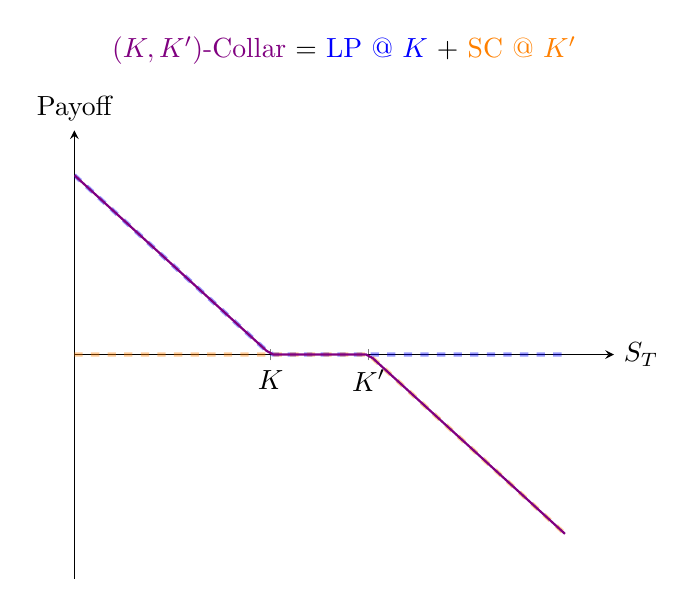
\begin{tikzpicture}[
declare function={
lc(\x) = (\x <= 3) * 0 + (\x > 3) * (\x - 3);
lp(\x) = (\x <= 2) * (2 - \x) + (\x > 2) * 0;
sp(\x) = (\x <= 2) * -(2 - \x) + (\x > 2) * 0;
sc(\x) = (\x <= 3) * 0 + (\x > 3) * -(\x - 3);
}
]
\begin{axis}[domain=0:5, ymin=-2.5, ymax=2.5, xmax=5.5, axis y line=left, axis x line=middle,
title={{\color{violet}\((K, K')\)-Collar} = {\color{blue}LP @ \(K\)} + {\color{orange}SC @ \(K'\)}},
title style={yshift=0.5cm}, xtick={2,3}, xticklabels={\(K\), \(K'\)},
ytick=\empty,
ylabel={Payoff},
ylabel style={at={(axis description cs:0,1)}, anchor=south, rotate=-90},
xlabel={\(S_T\)},
xlabel style={anchor=west}, samples=75
]
\addplot[blue, dashed, ultra thick, opacity=0.4] {lp(x)};
\addplot[orange, dashed, ultra thick, opacity=0.4] {sc(x)};
\addplot[violet, thick] {lp(x)+sc(x)};
\end{axis}
\end{tikzpicture}
\end{center}

\item The main usage of collar is to insure a long position in
\faIcon{apple-alt}.  Recall that a \emph{floor} is a way to hedge such risk (by
adding LP on top of long \faIcon{apple-alt}). The ``initial positive'' part of
payoff (P/L) of LP helps reducing the risk:

\begin{center}
\begin{tikzpicture}[
declare function={
lp(\x) = (\x <= 2) * (1.5-\x) + (\x > 2) * (-0.5);
la(\x) = (\x-2.2);
}
]
\begin{axis}[domain=0:5, ymin=-2.5, ymax=2.5, xmax=5.5, axis y line=left, axis x line=middle,
title={{\color{violet}Floor} = {\color{blue}Long \faIcon{apple-alt}} + {\color{orange}LP @ \(K\)}},
xtick={2}, xticklabel={\(K\)}, xticklabel style={yshift=0.7cm, xshift=0.2cm},
ytick={-2.2},
yticklabel={\(-S_0e^{rT}\)},
ylabel={P/L},
ylabel style={at={(axis description cs:0,1)}, anchor=south, rotate=-90},
xlabel={\(S_T\)},
xlabel style={anchor=west}, samples=75
]
\addplot[blue, thick, dashed, opacity=0.5]{la(x)};
\addplot[orange, thick, dashed, opacity=0.5]{lp(x)};
\addplot[violet, thick]{la(x)+lp(x)};
\draw[opacity=0.4, ForestGreen, line width=0.2cm, line cap=round, line join=round] (0,-0.7) -- (2,-0.7) -- (2.6,-0.1);
\node[ForestGreen] at (1.2,-0.4) {hedged \faIcon{shield-alt} risk};
\end{axis}
\end{tikzpicture}
\end{center}


\item However, for the floor, we need to pay the put option price \(P_0(K)\).
To reduce the initial expense, a \emph{collar} can be used instead of LP.
(Note that the payoff graph of collar also has an ``initial positive'' part.)

\begin{note}
We call ``long \faIcon{apple-alt} + collar'' as \defn{collared
\faIcon{apple-alt}}.  (We usually use this terminology for \emph{stock}:
collared stock.)
\end{note}

Since the time-0 value of a collar is \(P_0(K)-C_0(K')\), which is less than
\(P_0(K)\), this insurance is ``cheaper''. Of course there is no ``free lunch''
and the thing we give up is the profit ``potential'':
\begin{center}
\begin{tikzpicture}[
declare function={
lp(\x) = (\x <= 2) * (1.5-x) + (\x > 2) * -0.5;
sc(\x) = (\x <= 3) * 0.3 + (\x > 3) * -(x-3.3);
la(\x) = (\x-2.2);
}
]
\begin{axis}[
domain=0:5, ymin=-2.5, ymax=2.5, xmax=5.5, axis y line=left, axis x line=middle,
title={{\color{violet}Collared \faIcon{apple-alt}} = {\color{blue}Long \faIcon{apple-alt}} + {\color{orange}\((K, K')\)-Collar}},
title style={yshift=0.5cm},
xtick={2,3}, xticklabels={\(K\),\(K'\)}, xticklabel style={yshift=0.7cm, xshift=0.2cm},
ytick={-2.2},
yticklabel={\(-S_0e^{rT}\)},
ylabel={P/L},
ylabel style={at={(axis description cs:0,1)}, anchor=south, rotate=-90},
xlabel={\(S_T\)},
xlabel style={anchor=west}, samples=75,
legend entries={Collared \faIcon{apple-alt}, Floor},
legend style={legend pos=outer north east}
]
\addplot[violet, thick]{la(x) + lp(x) + sc(x)};
\addplot[opacity=0.4, magenta, thick]{la(x)+lp(x)};
\addplot[blue, thick, dashed, opacity=0.5]{la(x)};
\addplot[orange, thick, dashed, opacity=0.5]{lp(x) + sc(x)};
\draw[opacity=0.4, ForestGreen, line width=0.2cm, line cap=round, line join=round] (0,-0.4) -- (2,-0.4) -- (2.3,-0.1);
\end{axis}
\end{tikzpicture}
\end{center}
After taking a collar, the range of P/L gets restricted to a ``narrow''
range, just like a physical \emph{collar} put around the neck of an animal that
restricts its ``movement''. By varying \(K\) and \(K'\) (such that \(K'>K\) of
course), we can ``place'' the restriction at different ``locations'' and
control its ``strength'' (how ``narrow'').

\item The time-0 value of a collar \(P_0(K)-C_0(K')\) can be positive,
negative, or zero (depending on the choice of \(K\) and \(K'\)). If it is zero,
the collar is called \defn{zero-cost collar}.

\begin{intuition}
For zero-cost collar, the ``protection'' sources completely from the profit
potential given up, since we do not pay any money for this insurance.
\end{intuition}

\item However, if the strike price \(K\) specified is ``too high'', then it is
impossible to construct a zero-cost collar, as suggested by the following
result:
\begin{proposition}
\label{prp:k-high-no-zero-cost-collar}
If \(K\ge S_0e^{rT}\) (the no-arbitrage forward price), then for any \(K'>K\),
\[
C_0(K')<P_0(K)
\]
(so the time-0 value of the collar is always positive).
\end{proposition}
\begin{pf}
For any \(K'>K\),
\begin{align*}
P_0(K)&=C_0(K)+Ke^{-rT}-S_0&\text{(put-call parity)}\\
&>C_0(K')+{\color{violet}K}e^{-rT}-S_0&\text{(\cref{prp:call-put-price-strike-relationship})}\\
&\ge C_0(K')+{\color{violet}S_0e^{rT}}e^{-rT}-S_0\\
&=C_0(K').
\end{align*}
\end{pf}
\end{enumerate}
\subsection{Straddles}
\label{subsect:straddles}
\begin{enumerate}
\item Sometimes speculators are \emph{neither bullish nor bearish}, and
they speculate the \emph{volatility} instead. They are not speculating the
\emph{direction} of future price movement, but its \emph{magnitude} (large
movement \faIcon{arrow-right} high ``volatility''; small movement
\faIcon{arrow-right} low ``volatility'').
\item Some option strategies for volatility speculation are discussed in
\cref{subsect:straddles,subsect:strangles,subsect:butterfly-sprd}.
\item A \defn{straddle} is a combination of call and put on the same asset
\faIcon{apple-alt}, with the same strike price and expiration date.

\item The payoff graph of straddle:
\begin{center}
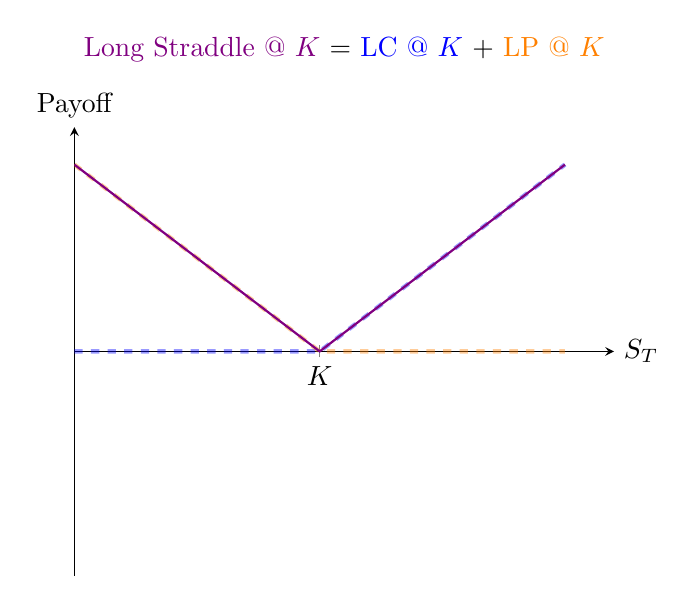
\begin{tikzpicture}[
declare function={
lc(\x) = (\x <= 2.5) * 0 + (\x > 2.5) * (\x - 2.5);
lp(\x) = (\x <= 2.5) * (2.5 - \x) + (\x > 2.5) * 0;
}
]
\begin{axis}[domain=0:5, ymin=-3, ymax=3, xmax=5.5, axis y line=left, axis x line=middle,
title={{\color{violet}Long Straddle @ \(K\)} = {\color{blue}LC @ \(K\)} + {\color{orange}LP @ \(K\)}},
title style={yshift=0.5cm}, xtick={2.5}, xticklabels={\(K\)},
ytick=\empty,
ylabel={Payoff},
ylabel style={at={(axis description cs:0,1)}, anchor=south, rotate=-90},
xlabel={\(S_T\)},
xlabel style={anchor=west}, samples=75
]
\addplot[blue, dashed, ultra thick, opacity=0.4] {lc(x)};
\addplot[orange, dashed, ultra thick, opacity=0.4] {lp(x)};
\addplot[violet, thick] {lc(x)+lp(x)};
\end{axis}
\end{tikzpicture}
\end{center}
\begin{note}
The ``shape'' of the graph looks like the act of ``straddling'' (sitting
astride), from ``top view''.
\end{note}


\item The time-0 price of a straddle is \(C_0+P_0\), which is positive. Hence,
its P/L graph can be obtained by shifting its payoff graph downward:
\begin{center}
\begin{tikzpicture}[
declare function={
lc(\x) = (\x <= 2.5) * 0 + (\x > 2.5) * (\x - 2.5);
lp(\x) = (\x <= 2.5) * (2.5 - \x) + (\x > 2.5) * 0;
}
]
\begin{axis}[domain=0:5, ymin=-3, ymax=3, xmax=5.5, axis y line=left, axis x line=middle,
title={{\color{violet}Long Straddle}},
title style={yshift=0.5cm}, xtick={2.5}, xticklabels={\(K\)},
ytick={-0.8}, yticklabels={\(-(C_0+P_0)e^{rT}\)},
ylabel={P/L},
ylabel style={at={(axis description cs:0,1)}, anchor=south, rotate=-90},
xlabel={\(S_T\)},
xlabel style={anchor=west}, samples=75
]
\addplot[violet, opacity=0.4, thick] {lc(x)+lp(x)};
\addplot[violet, thick] {lc(x)+lp(x)-0.8};
\draw[-Latex, brown] (1,1.3) -- (1,0.8);
\draw[-Latex, brown] (1.5,0.8) -- (1.5,0.3);
\draw[-Latex, brown] (3.5,0.8) -- (3.5,0.3);
\draw[-Latex, brown] (4,1.3) -- (4,0.8);
\end{axis}
\end{tikzpicture}
\end{center}

\item To speculate \emph{high} volatility (large future price movement in
either direction), one can long straddle.

\item On the other hand, if one want to speculate \emph{low} volatility (small
future price movement in either direction), one can \emph{short} straddle (SC @
\(K\) + SP @ \(K\)).

\item The payoff and P/L graphs of short straddle:
\begin{center}
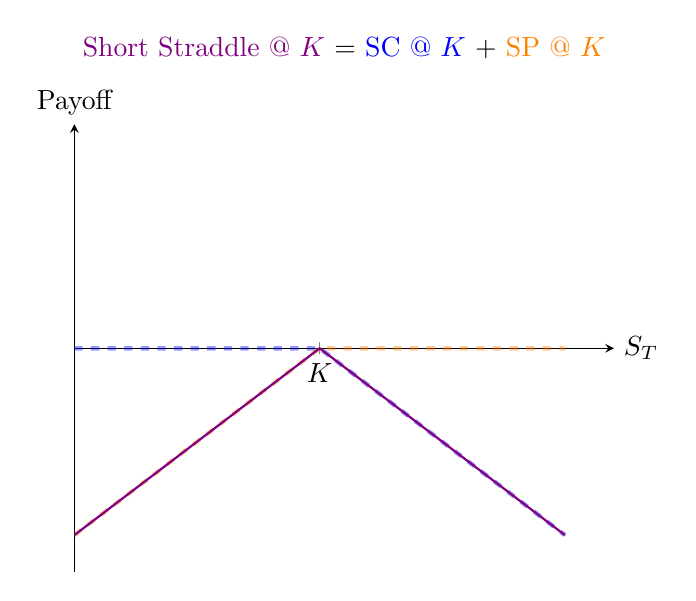
\begin{tikzpicture}[
declare function={
lc(\x) = (\x <= 2.5) * 0 + (\x > 2.5) * (\x - 2.5);
lp(\x) = (\x <= 2.5) * (2.5 - \x) + (\x > 2.5) * 0;
}
]
\begin{axis}[domain=0:5, ymin=-3, ymax=3, xmax=5.5, axis y line=left, axis x line=middle,
title={{\color{violet}Short Straddle @ \(K\)} = {\color{blue}SC @ \(K\)} + {\color{orange}SP @ \(K\)}},
title style={yshift=0.5cm}, xtick={2.5}, xticklabels={\(K\)},
ytick=\empty,
ylabel={Payoff},
ylabel style={at={(axis description cs:0,1)}, anchor=south, rotate=-90},
xlabel={\(S_T\)},
xlabel style={anchor=west}, samples=75
]
\addplot[blue, dashed, ultra thick, opacity=0.4] {-lc(x)};
\addplot[orange, dashed, ultra thick, opacity=0.4] {-lp(x)};
\addplot[violet, thick] {-lc(x)-lp(x)};
\end{axis}
\end{tikzpicture}

\begin{tikzpicture}[
declare function={
lc(\x) = (\x <= 2.5) * 0 + (\x > 2.5) * (\x - 2.5);
lp(\x) = (\x <= 2.5) * (2.5 - \x) + (\x > 2.5) * 0;
}
]
\begin{axis}[domain=0:5, ymin=-3, ymax=3, xmax=5.5, axis y line=left, axis x line=middle,
title={{\color{violet}Short Straddle}},
title style={yshift=0.5cm}, xtick={2.5}, xticklabels={\(K\)},
ytick={0.8}, yticklabels={\((C_0+P_0)e^{rT}\)},
ylabel={P/L},
ylabel style={at={(axis description cs:0,1)}, anchor=south, rotate=-90},
xlabel={\(S_T\)},
xlabel style={anchor=west}, samples=75
]
\addplot[violet, opacity=0.4, thick] {-lc(x)-lp(x)};
\addplot[violet, thick] {-lc(x)-lp(x)+0.8};
\draw[-Latex, brown] (1,-1.3) -- (1,-0.8);
\draw[-Latex, brown] (1.5,-0.8) -- (1.5,-0.3);
\draw[-Latex, brown] (3.5,-0.8) -- (3.5,-0.3);
\draw[-Latex, brown] (4,-1.3) -- (4,-0.8);
\draw[opacity=0.5, red, line width=0.2cm, line cap=round] (1,-0.7) -- (0,-1.7);
\draw[opacity=0.5, red, line width=0.2cm, line cap=round] (4,-0.7) -- (5,-1.7);
\node[red] () at (4.5,-0.3) {high risk \faIcon{exclamation-triangle}!};
\end{axis}
\end{tikzpicture}
\end{center}
\begin{warning}
A short straddle is highly risky and has \emph{unlimited} potential loss. This
strategy caused the collapse of \emph{Barings Bank}!
\end{warning}
\end{enumerate}
\subsection{Strangles}
\label{subsect:strangles}
\begin{enumerate}
\item A \emph{strangle} is another strategy for speculating volatility which is
``cheaper'' than straddle. To achieve a lower cost, call (put) option with
higher (lower) strike price is used, through which some profit potential is
given up.

\item A \((K-\Delta,K+\Delta)\)-\defn{strangle} is a combination of call and
put with strike prices \(K+\Delta\) and \(K-\Delta\) respectively, on the same
asset \faIcon{apple-alt}, with the same expiration date.

\begin{note}
The time-0 price of the \((K-\Delta,K+\Delta)\)-strangle is
\(C_0(K+\Delta)+P_0(K-\Delta)\), which is lower than the price of the straddle
@ \(K\): \(C_0(K)+P_0(K)\) since \(C_0(K+\Delta)<C_0(K)\) and
\(P_0(K-\Delta)>P_0(K)\) by \cref{prp:call-put-price-strike-relationship}.
\end{note}
\item The payoff and P/L graphs of long strangle:
\begin{center}
\begin{tikzpicture}[
declare function={
lc(\x) = (\x <= 3) * 0 + (\x > 3) * (\x - 3);
lp(\x) = (\x <= 2) * (2 - \x) + (\x > 2) * 0;
}
]
\begin{axis}[domain=0:5, ymin=-3, ymax=3, xmax=5.5, axis y line=left, axis x line=middle,
title={{\color{violet}Long \((K-\Delta,K+\Delta)\)-Strangle} = {\color{blue}LC @ \(K+\Delta\)} + {\color{orange}LP @ \(K-\Delta\)}},
title style={yshift=0.5cm}, xtick={2,3}, xticklabels={\(K-\Delta\),\(K+\Delta\)},
ytick=\empty,
ylabel={Payoff},
ylabel style={at={(axis description cs:0,1)}, anchor=south, rotate=-90},
xlabel={\(S_T\)},
xlabel style={anchor=west}, samples=75
]
\addplot[blue, dashed, ultra thick, opacity=0.4] {lc(x)};
\addplot[orange, dashed, ultra thick, opacity=0.4] {lp(x)};
\addplot[violet, thick] {lc(x)+lp(x)};
\end{axis}
\end{tikzpicture}

\begin{tikzpicture}[
declare function={
lc(\x) = (\x <= 3) * 0 + (\x > 3) * (\x - 3);
lp(\x) = (\x <= 2) * (2 - \x) + (\x > 2) * 0;
}
]
\begin{axis}[domain=0:5, ymin=-3, ymax=3, xmax=5.5, axis y line=left, axis x line=middle,
title={{\color{violet}Long Strangle}},
title style={yshift=0.5cm}, xtick={2,3}, xticklabels={\(K-\Delta\),\(K+\Delta\)},
xticklabel style={yshift=0.7cm},
ytick=\empty,
ylabel={P/L},
ylabel style={at={(axis description cs:0,1)}, anchor=south, rotate=-90},
xlabel={\(S_T\)},
xlabel style={anchor=west}, samples=75
]
\addplot[violet, thick, opacity=0.4] {lc(x)+lp(x)};
\addplot[violet, thick] {lc(x)+lp(x)-0.5};
\draw[->, brown] (1,0.95) -- (1,0.6);
\draw[->, brown] (1.5,0.45) -- (1.5,0.1);
\draw[->, brown] (3.5,0.45) -- (3.5,0.1);
\draw[->, brown] (4,0.95) -- (4,0.6);
\end{axis}
\end{tikzpicture}
\end{center}

\item The payoff and P/L graphs of short strangle:
\begin{center}
\begin{tikzpicture}[
declare function={
lc(\x) = (\x <= 3) * 0 + (\x > 3) * (\x - 3);
lp(\x) = (\x <= 2) * (2 - \x) + (\x > 2) * 0;
}
]
\begin{axis}[domain=0:5, ymin=-3, ymax=3, xmax=5.5, axis y line=left, axis x line=middle,
title={{\color{violet}Short \((K-\Delta,K+\Delta)\)-Strangle} = {\color{blue}SC @ \(K+\Delta\)} + {\color{orange}SP @ \(K-\Delta\)}},
title style={yshift=0.5cm}, xtick={2,3}, xticklabels={\(K-\Delta\),\(K+\Delta\)},
xticklabel style={yshift=0.7cm},
ytick=\empty,
ylabel={Payoff},
ylabel style={at={(axis description cs:0,1)}, anchor=south, rotate=-90},
xlabel={\(S_T\)},
xlabel style={anchor=west}, samples=75
]
\addplot[blue, dashed, ultra thick, opacity=0.4] {-lc(x)};
\addplot[orange, dashed, ultra thick, opacity=0.4] {-lp(x)};
\addplot[violet, thick] {-lc(x)-lp(x)};
\end{axis}
\end{tikzpicture}

\begin{tikzpicture}[
declare function={
lc(\x) = (\x <= 3) * 0 + (\x > 3) * (\x - 3);
lp(\x) = (\x <= 2) * (2 - \x) + (\x > 2) * 0;
}
]
\begin{axis}[domain=0:5, ymin=-3, ymax=3, xmax=5.5, axis y line=left, axis x line=middle,
title={{\color{violet}Short Strangle}},
title style={yshift=0.5cm}, xtick={2,3}, xticklabels={\(K-\Delta\),\(K+\Delta\)},
ytick=\empty,
ylabel={P/L},
ylabel style={at={(axis description cs:0,1)}, anchor=south, rotate=-90},
xlabel={\(S_T\)},
xlabel style={anchor=west}, samples=75
]
\addplot[violet, thick, opacity=0.4] {-lc(x)-lp(x)};
\addplot[violet, thick] {-lc(x)-lp(x)+0.5};
\draw[->, brown] (1,-0.95) -- (1,-0.6);
\draw[->, brown] (1.5,-0.45) -- (1.5,-0.1);
\draw[->, brown] (3.5,-0.45) -- (3.5,-0.1);
\draw[->, brown] (4,-0.95) -- (4,-0.6);
\end{axis}
\end{tikzpicture}
\end{center}

\item A comparison of P/L graphs of long strangle and long straddle:
\begin{center}
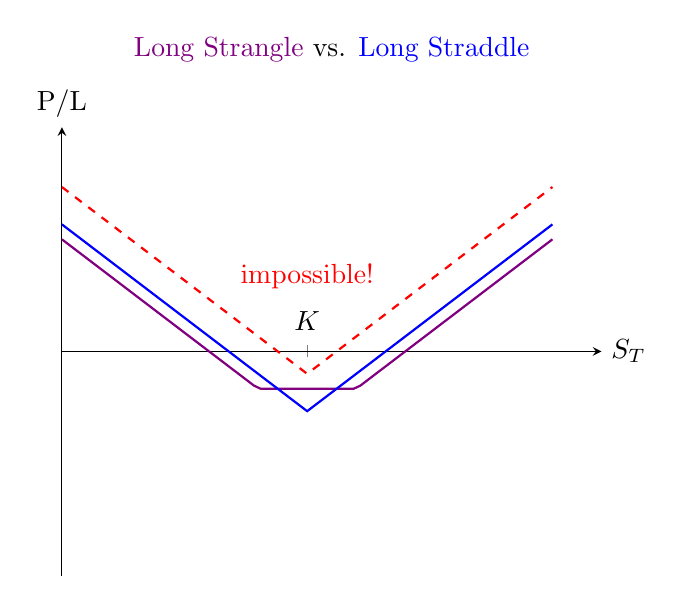
\begin{tikzpicture}[
declare function={
lc3(\x) = (\x <= 3) * 0 + (\x > 3) * (\x - 3);
lp2(\x) = (\x <= 2) * (2 - \x) + (\x > 2) * 0;
lc(\x) = (\x <= 2.5) * 0 + (\x > 2.5) * (\x - 2.5);
lp(\x) = (\x <= 2.5) * (2.5 - \x) + (\x > 2.5) * 0;
}
]
\begin{axis}[domain=0:5, ymin=-3, ymax=3, xmax=5.5, axis y line=left, axis x line=middle,
title={{\color{violet}Long Strangle} vs. {\color{blue}Long Straddle}},
title style={yshift=0.5cm}, xtick={2.5}, xticklabels={\(K\)},
xticklabel style={yshift=0.7cm},
ytick=\empty,
ylabel={P/L},
ylabel style={at={(axis description cs:0,1)}, anchor=south, rotate=-90},
xlabel={\(S_T\)},
xlabel style={anchor=west}, samples=75
]
\addplot[violet, thick] {lc3(x)+lp2(x)-0.5};
\addplot[blue, thick] {lc(x)+lp(x)-0.8};
\addplot[red, thick, dashed] {lc(x)+lp(x)-0.3};
\node[red] () at (2.5,1) {impossible!};
\end{axis}
\end{tikzpicture}
\end{center}
\begin{note}
Under the no-arbitrage principle, the graphs must cross each other. Otherwise,
arbitrage would be possible.
\end{note}
\end{enumerate}
\subsection{Butterfly Spreads}
\label{subsect:butterfly-sprd}
\begin{enumerate}
\item Recall that short straddle is highly risky. This suggests a need to
\emph{insure} the short straddle, and \emph{butterfly spread} is a strategy
that does this.

\item Recall: P/L graph of short straddle:
\begin{center}
\begin{tikzpicture}[
declare function={
lc(\x) = (\x <= 2.5) * 0 + (\x > 2.5) * (\x - 2.5);
lp(\x) = (\x <= 2.5) * (2.5 - \x) + (\x > 2.5) * 0;
}
]
\begin{axis}[domain=0:5, ymin=-3, ymax=3, xmax=5.5, axis y line=left, axis x line=middle,
title={{\color{violet}Short Straddle}},
title style={yshift=0.5cm}, xtick={2.5}, xticklabels={\(K\)},
ytick={0.8}, yticklabels={\((C_0+P_0)e^{rT}\)},
ylabel={P/L},
ylabel style={at={(axis description cs:0,1)}, anchor=south, rotate=-90},
xlabel={\(S_T\)},
xlabel style={anchor=west}, samples=75
]
\addplot[violet, thick] {-lc(x)-lp(x)+0.8};
\draw[opacity=0.5, red, line width=0.2cm, line cap=round] (1,-0.7) -- (0,-1.7);
\draw[opacity=0.5, red, line width=0.2cm, line cap=round] (4,-0.7) -- (5,-1.7);
\node[red] () at (4.5,-0.3) {high risk \faIcon{exclamation-triangle}!};
\end{axis}
\end{tikzpicture}
\end{center}
To insure the short straddle, we need \emph{both} ``initial positive'' and
``later positive'' parts for P/L, so \emph{long strangle} is a good candidate.

\begin{note}
Long straddle is another choice but it would just close out the short
straddle position (if they are both @ \(K\)), which is not very interesting.
\end{note}

\item A \((K-\Delta,K+\Delta)\)-\defn{butterfly spread} consists of ``short
straddle @ \(K\)'' + ``long \((K-\Delta,K+\Delta)\)-strangle''.

\item The payoff and P/L graphs of butterfly spread:
\begin{center}
\begin{tikzpicture}[ declare function={
lc3(\x) = (\x <= 3) * 0 + (\x > 3) * (\x - 3);
lp2(\x) = (\x <= 2) * (2 - \x) + (\x > 2) * 0;
lc(\x) = (\x <= 2.5) * 0 + (\x > 2.5) * (\x - 2.5);
lp(\x) = (\x <= 2.5) * (2.5 - \x) + (\x > 2.5) * 0;
}
]
\begin{axis}[domain=0:5, ymin=-3, ymax=3, xmax=5.5, axis y line=left, axis x line=middle,
title={{\color{violet}\((K-\Delta,K+\Delta)\)-Butterfly Spread} 
= {\color{blue}Short Straddle @ \(K\)} + {\color{orange}Long \((K-\Delta,K+\Delta)\)-Strangle)}},
title style={yshift=0.5cm}, xtick={2,3}, xticklabels={\(K-\Delta\),\(K+\Delta\)}, xticklabel style={above=0.2cm},
ytick=\empty,
ylabel={Payoff},
ylabel style={at={(axis description cs:0,1)}, anchor=south, rotate=-90},
xlabel={\(S_T\)},
xlabel style={anchor=west}, samples=75
]
\addplot[violet, thick] {lc3(x)+lp2(x)-lc(x)-lp(x)};
\addplot[orange, dashed, thick, opacity=0.4] {lc3(x)+lp2(x)};
\addplot[blue, dashed, thick, opacity=0.4] {-lc(x)-lp(x)};
\end{axis}
\end{tikzpicture}

\begin{tikzpicture}[
declare function={
lc3(\x) = (\x <= 3) * 0 + (\x > 3) * (\x - 3);
lp2(\x) = (\x <= 2) * (2 - \x) + (\x > 2) * 0;
lc(\x) = (\x <= 2.5) * 0 + (\x > 2.5) * (\x - 2.5);
lp(\x) = (\x <= 2.5) * (2.5 - \x) + (\x > 2.5) * 0;
}
]
\begin{axis}[domain=0:5, ymin=-3, ymax=3, xmax=5.5, axis y line=left, axis x line=middle,
title={{\color{violet}\((K-\Delta,K+\Delta)\)-Butterfly Spread}},
title style={yshift=0.5cm}, xtick={2,3}, xticklabels={\(K-\Delta\),\(K+\Delta\)},
xticklabel style={yshift=0.7cm},
ytick=\empty, ylabel={P/L},
ylabel style={at={(axis description cs:0,1)}, anchor=south, rotate=-90},
xlabel={\(S_T\)},
xlabel style={anchor=west}, samples=75,
]
\addplot[violet, thick] {lc3(x)+lp2(x)-lc(x)-lp(x) + 0.3};
\addplot[violet, thick, opacity=0.4] {lc3(x)+lp2(x)-lc(x)-lp(x)};
\draw[->, brown] (1,-0.45) -- (1,-0.2);
\draw[->, brown] (1.5,-0.45) -- (1.5,-0.2);
\draw[->, brown] (3.5,-0.45) -- (3.5,-0.2);
\draw[->, brown] (4,-0.45) -- (4,-0.2);
\end{axis}
\end{tikzpicture}
\end{center}
\begin{remark}
\item Either of payoff and P/L graphs looks like a ``butterfly'' flying away
(or towards you).
\item The P/L graph is obtained by shifting the payoff graph \emph{upward}
since P/L cannot be always nonpositive (alternatively, the strangle is cheaper
than the straddle \faIcon{arrow-right} time-0 value of butterfly spread is
negative).
\end{remark}
\item A comparison of P/L graphs of butterfly spread and short straddle:
\begin{center}
\begin{tikzpicture}[ declare function={
lc3(\x) = (\x <= 3) * 0 + (\x > 3) * (\x - 3);
lp2(\x) = (\x <= 2) * (2 - \x) + (\x > 2) * 0;
lc(\x) = (\x <= 2.5) * 0 + (\x > 2.5) * (\x - 2.5);
lp(\x) = (\x <= 2.5) * (2.5 - \x) + (\x > 2.5) * 0;
}
]
\begin{axis}[domain=0:5, ymin=-3, ymax=3, xmax=5.5, axis y line=left, axis x line=middle,
title={{\color{violet}\((K-\Delta,K+\Delta)\)-Butterfly Spread} 
= {\color{blue}Short Straddle @ \(K\)} + {\color{orange}Long \((K-\Delta,K+\Delta)\)-Strangle)}},
title style={yshift=0.5cm}, xtick={2,3}, xticklabels={\(K-\Delta\),\(K+\Delta\)}, xticklabel style={above=0.2cm},
ytick=\empty,
ylabel={Payoff},
ylabel style={at={(axis description cs:0,1)}, anchor=south, rotate=-90},
xlabel={\(S_T\)},
xlabel style={anchor=west}, samples=75
]
\addplot[violet, thick] {lc3(x)+lp2(x)-lc(x)-lp(x)};
\addplot[orange, dashed, thick, opacity=0.4] {lc3(x)+lp2(x)};
\addplot[blue, dashed, thick, opacity=0.4] {-lc(x)-lp(x)};
\end{axis}
\end{tikzpicture}

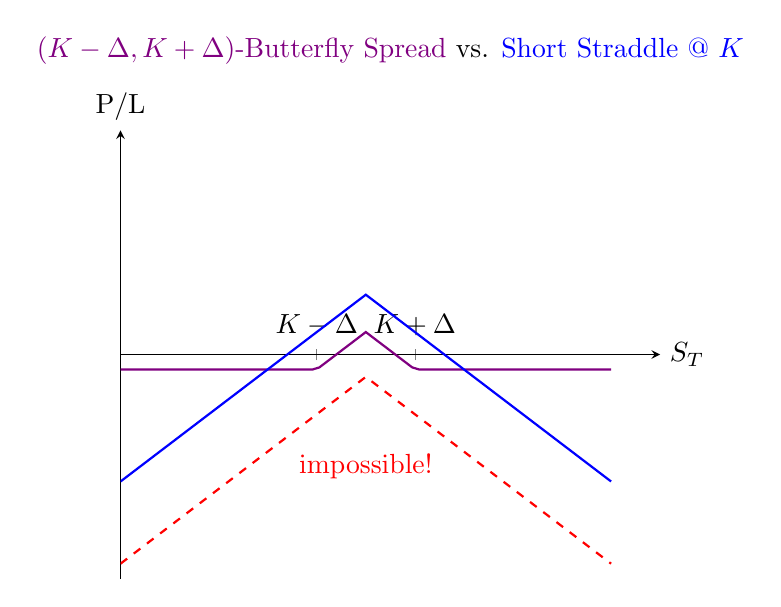
\begin{tikzpicture}[
declare function={
lc3(\x) = (\x <= 3) * 0 + (\x > 3) * (\x - 3);
lp2(\x) = (\x <= 2) * (2 - \x) + (\x > 2) * 0;
lc(\x) = (\x <= 2.5) * 0 + (\x > 2.5) * (\x - 2.5);
lp(\x) = (\x <= 2.5) * (2.5 - \x) + (\x > 2.5) * 0;
}
]
\begin{axis}[domain=0:5, ymin=-3, ymax=3, xmax=5.5, axis y line=left, axis x line=middle,
title={{\color{violet}\((K-\Delta,K+\Delta)\)-Butterfly Spread} vs. {\color{blue}Short Straddle @ \(K\)}},
title style={yshift=0.5cm}, xtick={2,3}, xticklabels={\(K-\Delta\),\(K+\Delta\)},
xticklabel style={yshift=0.7cm},
ytick=\empty, ylabel={P/L},
ylabel style={at={(axis description cs:0,1)}, anchor=south, rotate=-90},
xlabel={\(S_T\)},
xlabel style={anchor=west}, samples=75,
]
\addplot[violet, thick] {lc3(x)+lp2(x)-lc(x)-lp(x) + 0.3};
\addplot[blue, thick] {-lc(x)-lp(x)+0.8};
\addplot[red, dashed, thick] {-lc(x)-lp(x)-0.3};
\node[red] () at (2.5,-1.5) {impossible!};
\end{axis}
\end{tikzpicture}
\end{center}
\begin{note}
Again, under the no-arbitrage principle, the graphs must cross each other
(i.e., the short straddle graph cannot be ``below'' the ``butterfly''!).
\end{note}
\end{enumerate}


\printbibliography
\pdfbookmark[1]{Concepts and Terminologies}{concepts}
\printindex[def]
\pdfbookmark[1]{Results}{results}
\section*{Results}

\end{document}
